\documentclass[11pt,aps,preprint,nofootinbib,superscriptaddress,tightenlines]{revtex4-2}
\usepackage[T1]{fontenc}
\usepackage{amsmath,amssymb,mathtools}
\let\lambdabar\relax   % revtex defines it; newpxmath does too
\usepackage{newpxtext,newpxmath}
\usepackage{bm}
\usepackage[final]{microtype}
\usepackage{xcolor}
\usepackage{booktabs}
\usepackage{graphicx}
\usepackage{dsfont}
\usepackage[most]{tcolorbox}
\newcommand{\one}{\mathds{1}}
\newcommand{\pf}{\bm{\mathsf p}}
\newcommand{\avg}[1]{\langle #1\rangle}
\definecolor{darkblue}{RGB}{20,60,140}
\definecolor{accent}{RGB}{30,80,150}
\definecolor{tint}{RGB}{243,246,251}
% algorithms: a titled, tinted box
\newtcolorbox{algobox}[1]{enhanced, colback=tint, colframe=accent, boxrule=0.6pt, arc=2pt,
  left=6pt, right=6pt, top=4pt, bottom=4pt, fonttitle=\bfseries\small, coltitle=white,
  colbacktitle=accent, title={#1}, before skip=10pt, after skip=10pt}
% the central equations: a tinted panel with an accent rule on the left
\newtcolorbox{keyeq}{enhanced, colback=tint, frame hidden, borderline west={2pt}{0pt}{accent},
  sharp corners, left=4pt, right=4pt, top=0pt, bottom=0pt, before skip=6pt, after skip=6pt}
\usepackage[colorlinks=true,linkcolor=darkblue,citecolor=darkblue,urlcolor=darkblue]{hyperref}

\def\st{\begin{equation}}
\def\stp{\end{equation}}
\def\Eq#1{eq.~(\ref{#1})}
\def\Sect#1{Sect.~\ref{#1}}
\def\App#1{Appendix~\ref{#1}}
\def\Fig#1{Fig.~\ref{#1}}
\def\tr{\operatorname{tr}}
\let\oldparagraph\paragraph
\renewcommand{\paragraph}{\par\bigskip\oldparagraph}

\begin{document}

\title{The equilibrium of the positions: volume fluctuations and the pair correlation}
\author{D.~Teaney}
\affiliation{Department of Physics and Astronomy, Stony Brook University,
Stony Brook, New York 11794, USA}
\date{\today}

\begin{abstract}
In equilibrium the particle positions are distributed by the weight $\prod_aV_a^{(d+1)/2}\exp[(p/T)\sum_aV_a]$.  Expanded to second order in the
density of the particles, this weight gives the structure factor, the pair correlation and the volume fluctuations in closed form, with no
free parameter.  The pair correlation has the range of the kernel, $h$, not the spacing $a$; the spacing sets only its depth, through the number
of neighbours $\bar nh^2$.  The volume fluctuations are fixed by the same structure factor.  The theory agrees with hybrid Monte Carlo.
\end{abstract}

\maketitle

%=============================================================================
\section{The question and the answer}
\label{sec:answer}

Each particle has the volume
\st
V_a=\frac1{n_a},\qquad n_a=\sum_bW(\bm x_a-\bm x_b),
\label{volume}
\stp
the sum including $b=a$.  How large are the fluctuations of $V_a$ in equilibrium, how are they related to the pair correlation $g(r)$, and is
the scale of $g(r)$ the kernel size $h$ or the spacing $a$?  With $\bar n=N/L^2$ the mean density and
\st
S(\bm k)=\frac1N\Big\langle\Big|\sum_ae^{-i\bm k\cdot\bm x_a}\Big|^2\Big\rangle,\qquad
S(k)=1+\bar n\int d^2r\,e^{-i\bm k\cdot\bm r}\,[g(r)-1],
\stp
the answer is three formulas.
\begin{keyeq}
\st
S(k)=\frac{1}{1+2\alpha\,\widetilde W(1-\tfrac12\widetilde W)+2\sigma\,\widetilde W(1-\widetilde W)},\qquad \alpha=\frac{d+1}2,\qquad \sigma=\frac{p}{T\bar n},\qquad d=2,
\label{Sk}
\stp
\st
\frac{\avg{n_a}}{\bar n}=1+\frac1{\bar n}\int\!\frac{d^2k}{(2\pi)^2}\,\widetilde W(k)\,S(k),\qquad
\frac{\avg{\delta V_a^2}}{V^2}=\frac1{\bar n}\int\!\frac{d^2k}{(2\pi)^2}\,\widetilde W(k)^2\,S(k),
\label{Vfluct}
\stp
\end{keyeq}
with $\widetilde W(k)$ the Fourier transform of the kernel ($\widetilde W(0)=1$) and $\sigma$ the pressure over the temperature of the bath, both constants of the (canonical) ensemble, times the mean particle volume
$V=1/\bar n$: not the fluctuating $p_a$, $T_a$, $V_a$ of the particles.  The volume variance is normalized by the same $V$.  \Eq{Sk} is the Gaussian (random-phase) approximation, valid when a particle has many
neighbours; the first of \Eq{Vfluct} is exact; the second treats the density seen by a particle as that seen by a fixed point.

\paragraph{The parameter.}  The point: the equation of state enters only through $\sigma$, the one number the fluid contributes to the weight of
the positions.  It comes from the weight of a single particle.  At the temperature $T$ of the bath, at rest, a particle with entropy $s_a$, momentum $\bm m_a$
and volume $V_a$ has the weight $e^{\Phi_a}$, with
\st
\Phi_a=s_a-\frac{e_a(s_a,\bm m_a,V_a)}{T}
\label{Phia}
\stp
the Massieu function of the particle (\texttt{eqstart.tex}, eq.~(Phi) there, where a moving bath adds $+\bm v\cdot\bm m_a/T$).  Its maximum over $s_a$ and $\bm m_a$ is at
$T_a=T$, $\bm m_a=0$, where $p_a=p(T)$, and is the value of $p_aV_a/T_a$ there; at the mean volume $V=1/\bar n$ this is
\st
\sigma\equiv\max_{s_a,\bm m_a}\Phi_a\Big|_{V_a=V}=\frac{p(T)\,V}{T}=\frac p{T\bar n} ,
\stp
the one-particle form of Israel's thermodynamic potential, $\Phi^\mu=s^\mu+\beta_\nu T^{\mu\nu}=p\beta^\mu$, whose time component is $p/T$ (\Sect{sec:weight}, \App{app:single}).  It is
not the average of $p_aV_a/T_a$, which differs at order $1/s_a$.  $\sigma$ is the logarithm of the grand partition function of the fluid in one particle
volume; for a gas of quanta it is about the number of quanta in that volume.  At rest $Ts=e+p$ and $s=dp/dT$, so
\st
\sigma=\frac{s(T)V}{d\ln p/d\ln T}=\frac{c_s^2}{1+c_s^2}\,s(T)V=\frac{s}{s+C_V}\,s(T)V ,
\label{sigma}
\stp
the last two for a constant speed of sound, $c_s^2=s/C_V$, with $C_V=T\,ds/dT$ the heat capacity per unit volume.  Here $s(T)V$ is the entropy of the bath
in one particle volume, and $s$ and $C_V$ are also those of the bath, at its temperature $T$.  The hybrid Monte Carlo runs of
\Sect{sec:test} are for the conformal fluid in $d=2$, $c_s^2=1/2$, so that $\sigma=s(T)V/3$ (\texttt{dimension.tex}; the version of 2026-11-17 had
$c_s^2=1/3$).  They sample the canonical ensemble at a bath temperature $T_0$, and are labelled by its
\st
\sigma(T_0)=\frac{p(T_0)}{T_0\bar n}=3.89,\ 16.4,\ 179 ,
\stp
which start from the entropy per particle $s_a=16$, $54$, $541$ on the lattice (\Sect{sec:test}).

\paragraph{The scale.}  In units of $h$ the kernel is fixed, $\widetilde W=\widetilde W(kh)$, so
\begin{keyeq}
\st
g(r)-1=\frac{1}{\bar nh^2}\,F\Big(\frac rh;\,\sigma\Big),\qquad
\frac{\avg{\delta V_a^2}}{V^2}=\frac{1}{\bar nh^2}\,G(\sigma),\qquad \bar nh^2=\frac2{\sqrt3}\Big(\frac ha\Big)^2 .
\label{scaling}
\stp
\end{keyeq}
The pair correlation has the range $h$; the spacing enters only through the number of neighbours $\bar nh^2$, which sets the depth of the
correlation hole and the size of the volume fluctuations.  Both fall as $(a/h)^2$ in the continuum limit.

%=============================================================================
\section{The weight of the positions}
\label{sec:weight}

Integrating the energies and momenta out of the equilibrium at fixed positions (\texttt{equilibrium\_positions.tex}, \texttt{scheme.tex})
leaves
\st
P(\{\bm x\})\propto\prod_aV_a^{\alpha}\,\exp\Big[\frac pT\sum_aV_a\Big],\qquad \alpha=\frac{d+1}2,
\label{Px}
\stp
with $V_a$ from \Eq{volume}.  The exponential rewards a large total volume; the prefactor is the Gaussian width of the $d+1$ integrated
variables of each particle (the entropy and the $d$ components of the momentum), whence the exponent $\alpha=(d+1)/2$.  Write the sum over particles as an integral over the microscopic density $\rho(\bm x)=\sum_a\delta(\bm x-\bm x_a)$,
\st
\sum_aV_a=\int d^2x\,\frac{\rho(\bm x)}{n(\bm x)},\qquad \sum_a\ln V_a=-\int d^2x\,\rho(\bm x)\ln n(\bm x),\qquad n=W*\rho .
\label{functional}
\stp

\paragraph{What the total volume penalizes.}  Expand about the uniform density, $\rho=\bar n+\delta\rho$.  To second order (\App{app:expand})
\st
\sum_aV_a=L^2-\frac1{\bar n^2L^2}\sum_{\bm k}\widetilde W(k)\big[1-\widetilde W(k)\big]\,|\delta\rho_{\bm k}|^2 .
\label{V2}
\stp
The cost vanishes at both ends.
\begin{itemize}
\item $kh\to0$: a density that varies slowly on the scale $h$ is seen exactly by the kernel, $n=\rho$, and $\sum_aV_a=\int\rho/\rho=L^2$.
  Moving particles at long wavelength relabels the fluid; it does not change it.
\item $kh\to\infty$: the kernel averages the fluctuation away, and $n$ does not see it.
\end{itemize}
Only fluctuations on the scale of the kernel cost entropy, at the rate $\sigma=p/(T\bar n)$ per particle.  Together with the entropy of placing $N$
points (the $1$ in \Eq{Sk}) and the prefactor of \Eq{Px} (the term $2\alpha\widetilde W(1-\widetilde W/2)$), this Gaussian weight gives \Eq{Sk}.  Because
$0\le\widetilde W\le1$ for the Wendland kernels, every mode is stable; a kernel with $\widetilde W<0$ at some $k$ would be unstable there.

%=============================================================================
\section{The structure factor and the pair correlation}
\label{sec:sk}

\Eq{Sk} has three regions.
\st
S(k)\approx\begin{cases}
\dfrac{1}{1+\alpha+\sigma\mu_2k^2/2},& kh\ll1,\\[2ex]
\dfrac1{2\sigma\,\widetilde W(1-\widetilde W)},& kh\sim1,\\[2ex]
1,& \widetilde W\ll1/\sigma,
\end{cases}
\label{regions}
\stp
with $\mu_2=\int d^2r\,r^2W\approx0.56\,h^2$.  On the scale of the kernel the positions are nearly incompressible, $S\sim1/\sigma$; toward long
wavelengths $S$ rises, because there the volumes do not constrain the positions, to $S(0)=1/(1+\alpha)=2/5$ set by the prefactor alone; at short distances the
particles are free.  This is the rise toward small $k$ seen in \texttt{equilibrium\_positions.tex}.

The pair correlation is the Fourier transform,
\st
\bar n\,[g(r)-1]=\int\frac{d^2k}{(2\pi)^2}\,J_0(kr)\,[S(k)-1] .
\stp
$S-1\approx-1$ over the region $kh\sim1$ where the kernel is stiff, so $g$ has a correlation hole of radius about $0.6h$ and depth $\sim1/(\bar nh^2)$.  It
holds a deficit of $1-S(0)=\alpha/(1+\alpha)=3/5$ of a particle (\Fig{fig:gr}).  At large $\sigma$ the hole is deep at $r\lesssim0.2h$, $g(0)$ becomes negative in the
Gaussian theory, and the theory fails there; outside it holds.

%=============================================================================
\section{The volume fluctuations}
\label{sec:volume}

\paragraph{The mean.}  The density at a particle counts the particle itself, $W(0)$, and its neighbours, $\bar n\int g\,W$:
\st
\avg{n_a}=W(0)+\bar n\int d^2r\,g(r)\,W(r)=\bar n+\int\frac{d^2k}{(2\pi)^2}\,\widetilde W(k)\,S(k),
\label{mean}
\stp
exactly.  For random positions ($S=1$) the excess is the self term, $W(0)/\bar n\approx0.12$ at $h/a=2$.  The correlation hole removes most of it:
the particles keep their neighbours away to make room for their own kernel.

\paragraph{Why $\avg{n_a}\neq\bar n$.}  There are two averages.  The average over space is exactly $\bar n$, since $\int d^2x\,n=N\widetilde W(0)=N$.  The
average over the particles samples $n$ where the particles are:
\st
\avg{n_a}=\frac1N\int d^2x\,\rho\,n=\bar n+\frac1N\int d^2x\,\delta\rho\,\delta n ,
\stp
and the covariance of $\rho$ and $n$ is $\int d^2k\,\widetilde W S/(2\pi)^2>0$: each particle sits on its own kernel.  In position space
\st
\frac{\avg{n_a}-\bar n}{\bar n}=\frac1{\bar n}\Big[W(0)-\bar n\int d^2r\,[1-g(r)]\,W(r)\Big] ,
\stp
the self term less the part of the hole that overlaps the kernel.  The hole obeys the compressibility sum rule,
\st
\bar n\int d^2r\,[g(r)-1]=S(0)-1=-\frac{\alpha}{1+\alpha} ,
\label{sumrule}
\stp
which fixes its total deficit but not its overlap with $W$, so the cancellation of the self term is only partial.

\paragraph{The excess as a scaling function.}  As in \Eq{scaling},
\st
\frac{\avg{n_a}}{\bar n}=1+\frac{G_1(\sigma)}{\bar nh^2},\qquad G_1(\sigma)=h^2\int\frac{d^2k}{(2\pi)^2}\,\widetilde W(k)\,S(k),
\stp
and the mean volume follows from the same integrals,
\st
\avg{V_a}\bar n=1-\frac1{\bar n}\int\frac{d^2k}{(2\pi)^2}\,\widetilde W\big(1-\widetilde W\big)\,S ,
\stp
which is $\bar n/\avg{n_a}$ corrected by the variance (at $h/a=2$, $\sigma=4$: $0.960\times1.017=0.976$).  The excess falls as $1/\bar nh^2$ at fixed $\sigma$, and
roughly as $1/\sigma$ at fixed $\bar nh^2$ (Table~\ref{tab:G1}).

\begin{table}[h]
\caption{$G_1(\sigma)$, the excess of the mean particle density times $\bar nh^2$, and $\avg{n_a}/\bar n$ for C2 at the parameters of the runs.  The first row is
random positions, $G_1=W(0)h^2$; the second, $\sigma=0$, the measure alone.}
\label{tab:G1}
\begin{ruledtabular}
\begin{tabular}{c ccc ccc}
 & \multicolumn{3}{c}{$G_1$} & \multicolumn{3}{c}{$\avg{n_a}/\bar n$, C2} \\
$\sigma$ & C2 & C4 & C6 & $h/a=2$ & $3$ & $4$ \\
\colrule
$S=1$ & 0.557 & 0.716 & 0.887 & 1.121 & 1.054 & 1.030 \\
0     & 0.302 & 0.380 & 0.469 & 1.065 & 1.029 & 1.016 \\
4     & 0.195 & 0.239 & 0.293 & 1.042 & 1.019 & 1.011 \\
10    & 0.136 & 0.162 & 0.197 & 1.029 & 1.013 & 1.007 \\
13.5  & 0.118 & 0.139 & 0.168 & 1.026 & 1.011 & 1.006 \\
100   & 0.037 & 0.038 & 0.044 & 1.008 & 1.004 & 1.002 \\
135   & 0.030 & 0.031 & 0.035 & 1.0065 & 1.0029 & 1.0016 \\
$10^3$ & 0.0082 & 0.0069 & 0.0073 & 1.0018 & 1.0008 & 1.0004 \\
$10^4$ & 0.0018 & 0.0012 & 0.0011 & 1.0004 & 1.0002 & 1.0001 \\
\end{tabular}
\end{ruledtabular}
\end{table}

\paragraph{The variance.}  To the same order, $\delta n_a=(W*\delta\rho)(\bm x_a)$ and $\delta V_a/V=-\delta n_a/\bar n$, which gives the second of
\Eq{Vfluct}: the volume fluctuations are the density fluctuations filtered twice by the kernel.  In position space,
\st
\frac{\avg{\delta V_a^2}}{V^2}=\frac1{\bar n}\Big[(W*W)(0)+\bar n\int d^2r\,(W*W)(r)\,[g(r)-1]\Big]:
\stp
the Poisson value $(W*W)(0)/\bar n$, reduced by the correlation hole weighted by the overlap of two kernels.  The dominant region is $kh\sim1$,
where $S\approx1/(2\sigma\widetilde W(1-\widetilde W))$, so
\st
\frac{\avg{\delta V_a^2}}{V^2}\approx\frac{1}{2\sigma\bar n}\int\frac{d^2k}{(2\pi)^2}\,\frac{\widetilde W}{1-\widetilde W}
\sim\frac1\pi\,\frac{\ln\sigma}{\sigma\,\bar nh^2}=\frac1\pi\,\frac{\ln\sigma}{p\,h^2/T},
\label{Vlog}
\stp
the logarithm from the long wavelengths, cut off where $S$ reaches $S(0)$ (or by the box).  The fluid enters through $p\,h^2/T$, the pressure over the temperature times the area of a
kernel; the logarithm belongs to the particles.  The estimate $1/\sigma$ of
\texttt{equilibrium\_positions.tex} treats each volume as independent; the volumes are correlated over the kernel, and the fluctuations are
smaller by the number of neighbours.

\begin{table}[h]
\caption{The predictions \Eq{Vfluct}, infinite box, at three values of $\sigma$ (the theory depends on $\sigma$ and $\bar nh^2$ only).}
\label{tab:predict}
\begin{ruledtabular}
\begin{tabular}{cc ccc ccc}
 & & \multicolumn{3}{c}{$\avg{V_a}\bar n$} & \multicolumn{3}{c}{$10^3\avg{\delta V_a^2}/V^2$} \\
$h/a$ & $\bar nh^2$ & $\sigma=4$ & $13.5$ & $135$ & $4$ & $13.5$ & $135$ \\
\colrule
2 & 4.62 & 0.976 & 0.985 & 0.996 & 17.2 & 10.0 & 2.09 \\
3 & 10.4 & 0.989 & 0.993 & 0.998 & 7.63 & 4.45 & 0.93 \\
4 & 18.5 & 0.994 & 0.996 & 0.999 & 4.29 & 2.50 & 0.52 \\
\end{tabular}
\end{ruledtabular}
\end{table}

%=============================================================================
\section{Against hybrid Monte Carlo}
\label{sec:test}

Hybrid Monte Carlo (\texttt{examples/volume\_fluctuations.jl}, the default Liouville measure, 200 updates from the lattice, the first third
discarded) in a box $L=9h$, at $h/a=2$, $3$, $4$; acceptance $0.98$--$0.99$.

\paragraph{The temperature of the runs, $T_0$.}  The point: every constant of the theory ($\sigma$, $C_V$, $e+p$) is evaluated at the temperature of the
ensemble that hybrid Monte Carlo samples.  That temperature, $T_0$, is defined from the parameters of the initial state, and it is not the temperature
$T(S_0)$ that a continuum fluid with the initial entropy density $S_0$ would have.  The procedure is:
\begin{enumerate}
\item \emph{Initialize} with the parameters $S_0$, $L$, $h$, $a$: $N$ particles on a hexagonal lattice, at rest, each with the volume of a single particle,
  \st
  V=\frac{L^2}N=\frac{\sqrt3}2\,a^2 ,
  \stp
  and the entropy $s_a=S_0V$, where
  \st
  S_0=\frac{\sum_as_a}{L^2}
  \stp
  is the initial entropy density (capital $S$ for an entropy density, as in \App{app:expand} and the code, \texttt{S0}, \texttt{S\_smooth}).  The total initial energy
  is $L^2e(S_0)$, with $e(S)$ the energy density at rest as a function of the entropy density.  The initial entropy per particle is $s_a=16$, $54$, $541$.
\item \emph{Define $T_0$} from these parameters: the temperature at which the canonical mean energy of the particles, on the same lattice, equals the initial energy,
  \begin{keyeq}
  \st
  N\avg{e_a}_{T_0}\equiv L^2\,e(S_0),\qquad \avg{e_a}_T=\frac{\int ds\,d^2\bm m\;e\,e^{s-e/T}}{\int ds\,d^2\bm m\;e^{s-e/T}}\quad\text{at }V_a=V .
  \label{T0def}
  \stp
  \end{keyeq}
  $\avg{e_a}_T$ is computed exactly from the single-particle partition function $Z_a(V)$, by quadrature (\texttt{beta\_from\_averages} in \texttt{src/measure.jl}).
  The volume enters $\avg{e_a}$; on the lattice every particle has $V_a=V$.
\item \emph{Create the ensemble}: hybrid Monte Carlo samples the canonical ensemble (positions, entropies, momenta) at the temperature $T_0$.  The positions
  move and the $V_a$ fluctuate, but $T_0$ stays fixed.  $T_0$ is recorded in each run (\texttt{T0}).
\end{enumerate}

\paragraph{Why $T_0$ is below $T(S_0)$.}  The mean energy of a particle at temperature $T$ is not just its share $e_0=V\,e(T)$ of the continuum energy: each
particle also holds the energy of its own thermal fluctuations, of its entropy and of its momentum (\App{app:expand}, \Eq{intrinsic}),
\st
\avg{e_a}_T=e_0+\Delta e,\qquad e_0=V\,e(T) .
\label{eparticle}
\stp
By $\avg{e_a}=T^2\partial_T\ln Z_a$ and the Gaussian $Z_a$ of \App{app:expand}, \Eq{Zgauss}, whose widths are $C_VV$ (entropy) and $T(e+p)V$ (each momentum component),
\st
\Delta e=T^2\frac{d}{dT}\ln\big[C_V\,(T(e+p))^d\big]^{1/2}
=\frac T2\Big[\frac{d\ln C_V}{d\ln T}+d\,\frac{d\ln\big(T(e+p)\big)}{d\ln T}\Big] .
\label{Deltae}
\stp
The widths grow with the temperature, so heating a particle puts energy into its fluctuations as well as into $e_0$.  For the conformal fluid in $d=2$,
$p\propto T^3$ ($C_V\propto T^2$, $T(e+p)\propto T^4$),
\st
\Delta e=\frac T2\,(2+2\times4)=5\,T,\qquad \frac{\Delta e}{e_0}=\frac{5\,T}{\tfrac23\,s(T)V\,T}\simeq\frac{7.5}{s_a},
\stp
a correction of order $1/s_a$ (the exact quadrature, \App{app:misses}, gives $\Delta e=5.0\,T$ at large $s_a$ and $4.7\,T$ at $s(T)V=12$).  It is not a positional
effect: $T_0$ is defined on the lattice, where all the volumes are equal.  Since the initial energy $L^2e(S_0)$ must also supply $N\Delta e$, \Eq{T0def} gives
$e(T_0)<e(S_0)$:
\st
\frac{T_0}{T(S_0)}=0.855,\ 0.955,\ 0.996\qquad(s_a=16,\ 54,\ 541),
\stp
most at the smallest $s_a$.

\paragraph{The ensemble at $T_0$.}  The point: the theory is a function of $\sigma$ at the temperature of the ensemble, so the runs are labelled by
\st
\sigma(T_0)=\frac{p(T_0)}{T_0\bar n}=\frac13\,s(T_0)V=3.89,\ 16.4,\ 179\qquad(s_a=16,\ 54,\ 541),
\stp
not by the $\sigma$ of the start, $s_a/3=5.3$, $18$, $180$.  Its entropy is not that of the initial state either.  The entropy density of the continuum at $T_0$,
$s(T_0)=S_0\,(T_0/T(S_0))^2$, is $0.730$, $0.912$, $0.992$ of $S_0$; the mean entropy per particle of the ensemble, $\avg{s_a}=1.26$, $1.07$, $1.01$ times $s(T_0)V$
(each particle's fluctuations add to its mean, \App{app:misses}), is $0.92$, $0.97$, $1.00$ of the initial $S_0V$.

\paragraph{The theory in the figures.}  In the figures the solid lines are \Eq{Sk} at $\sigma(T_0)$, with $\alpha=3/2$, and the dashed lines (same colour) the
improved theory: the weight of a particle at fixed volume integrated exactly instead of by its saddle point (\App{app:misses}, \texttt{statics.tex}), so that
\Eq{Sk} keeps its form with $\alpha,\sigma\to\alpha_{\rm eff},\sigma_{\rm eff}$, the effective phase-space exponent and volume coefficient of a particle, from the
exact $\ln Z_a(V)$.  The table gives both.  Sums over the modes of the box (the box lowers the variance by up to $33\%$ at $\sigma=179$, through the logarithm of
\Eq{Vlog}).  Analysis: \texttt{examples/volume\_fluctuations.py}, with \texttt{examples/statics\_theory.py}.

\begin{figure}[h]
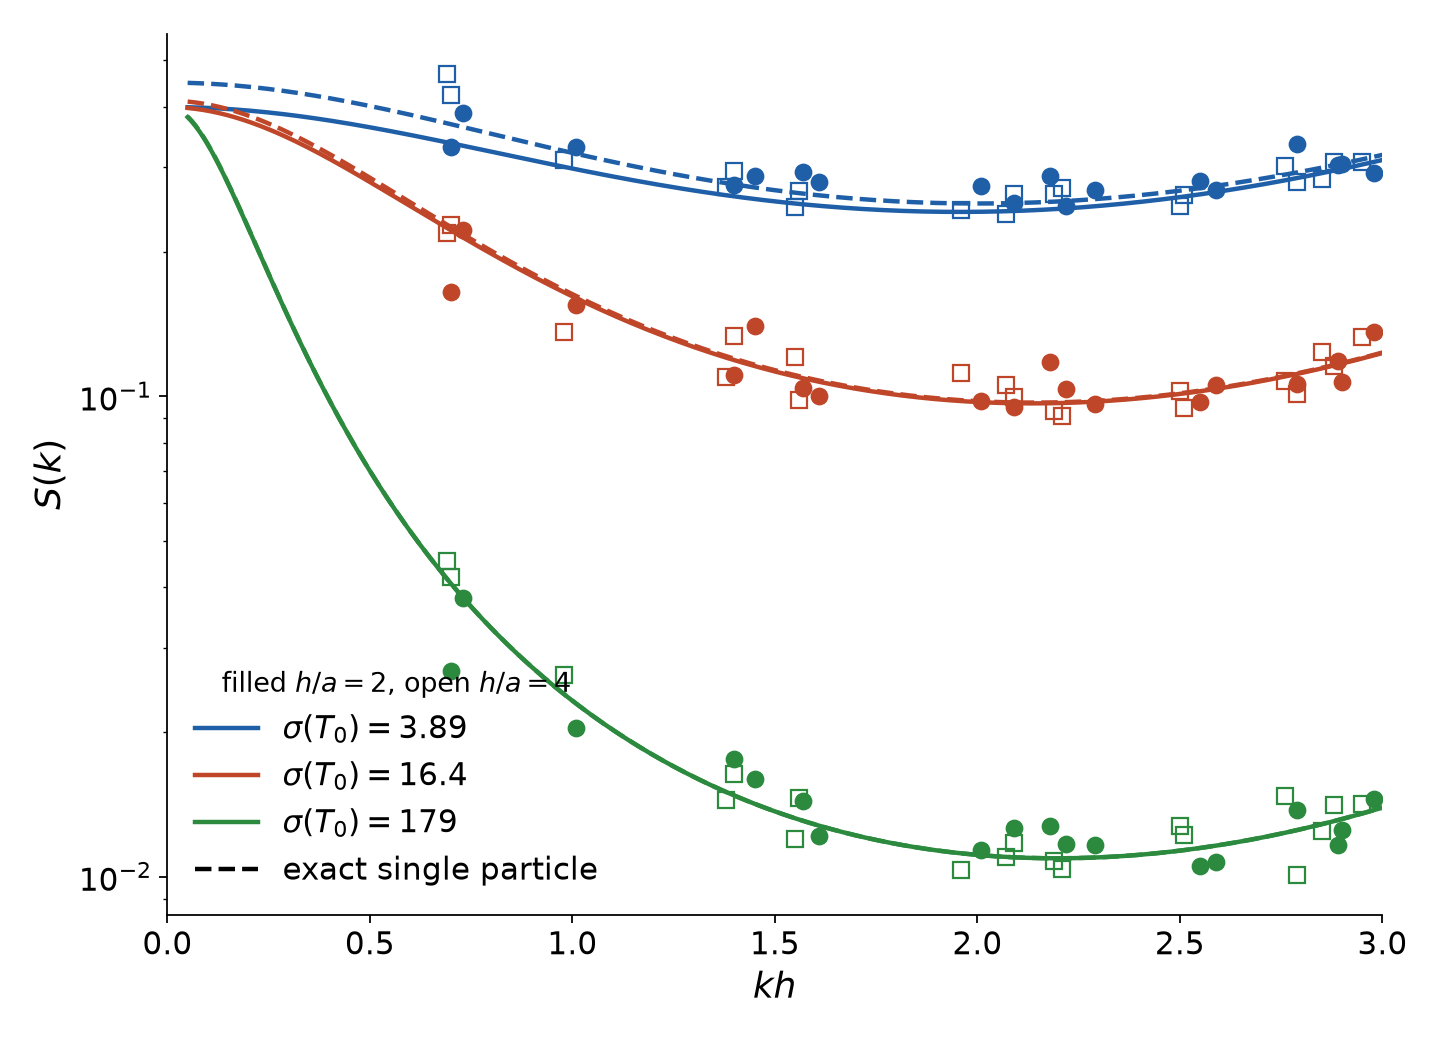
\includegraphics[width=0.7\textwidth]{figs/equilibrium_Sk.png}
\caption{$S(k)$, hybrid Monte Carlo (points), $L=9h$, at $h/a=2$ (filled) and $4$ (open), against \Eq{Sk} at $\sigma(T_0)$ (solid) and the improved theory
with the exact single particle (dashed).  One curve per $\sigma$: the theory does not depend on $h/a$.}
\label{fig:sk}
\end{figure}

\begin{figure}[h]
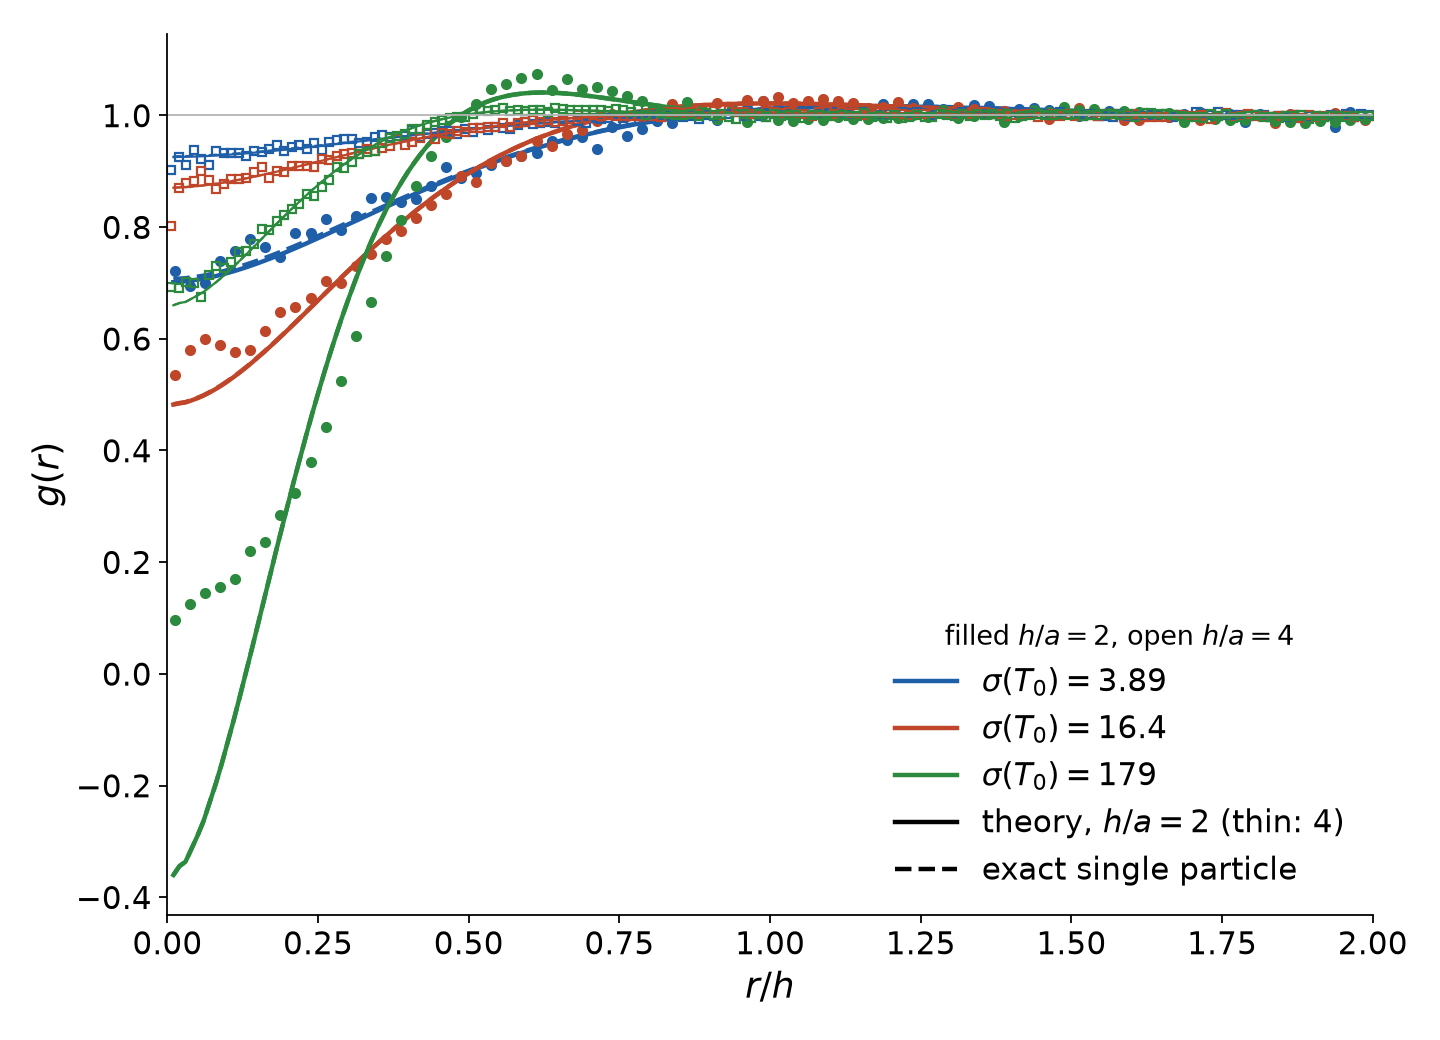
\includegraphics[width=0.7\textwidth]{figs/equilibrium_gr.png}
\caption{$g(r)$, hybrid Monte Carlo (points) at $h/a=2$ (filled) and $4$ (open), against the Gaussian theory at $\sigma(T_0)$ (solid; thick $h/a=2$, thin $4$) and the
improved theory with the exact single particle (dashed).}
\label{fig:gr}
\end{figure}

\begin{figure}[h]
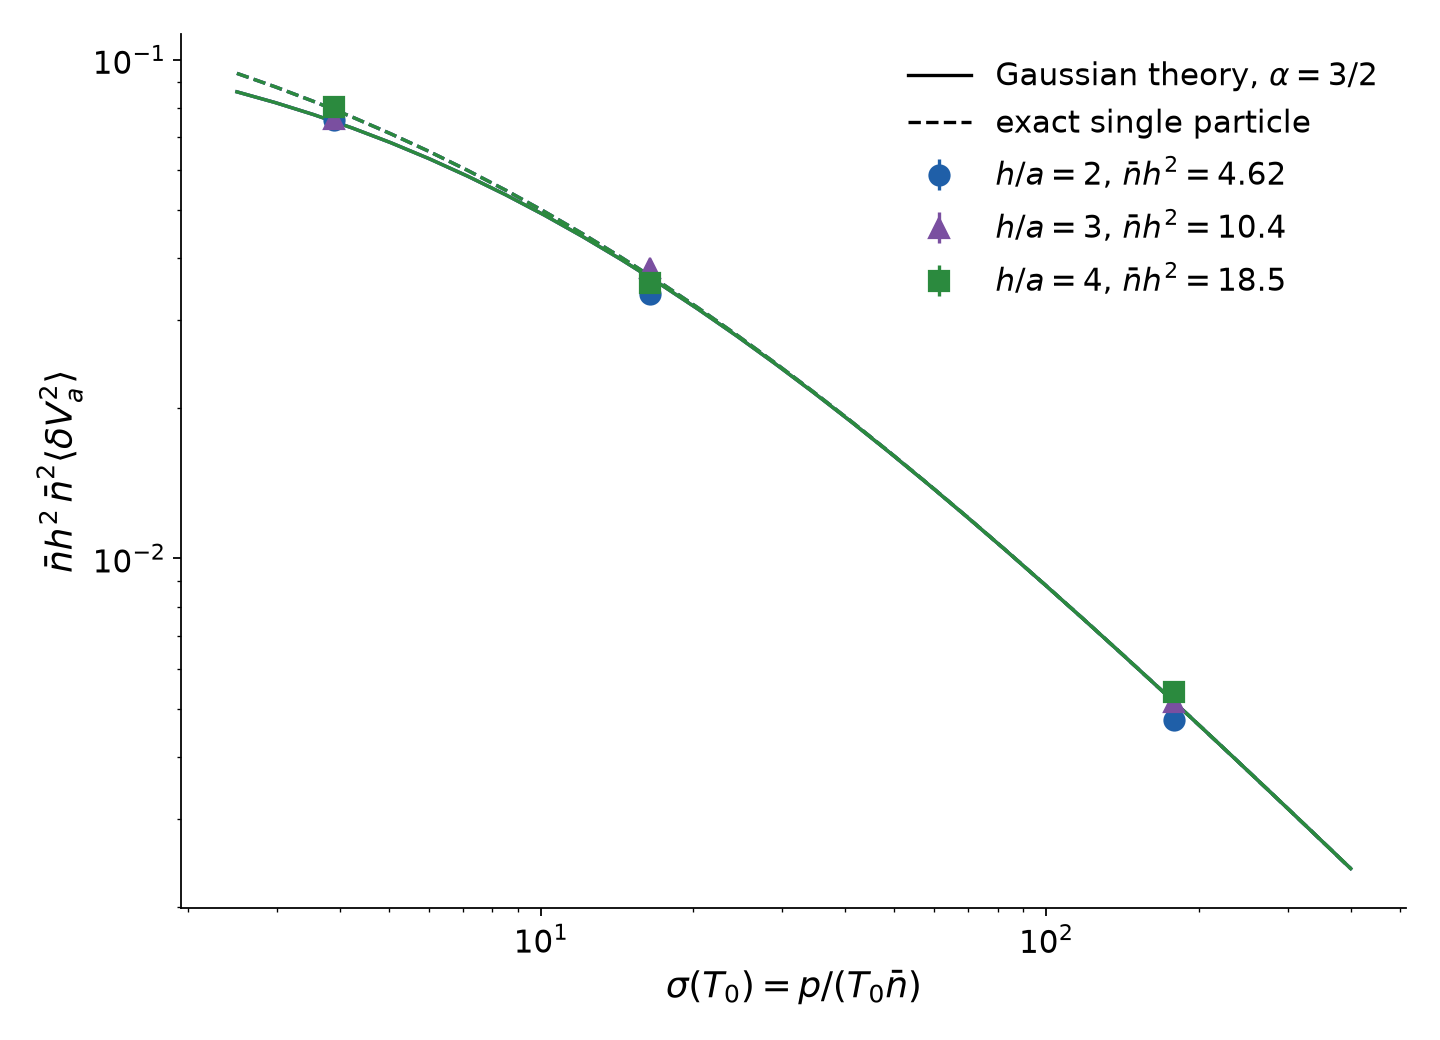
\includegraphics[width=0.7\textwidth]{figs/equilibrium_volvar.png}
\caption{The volume variance times the number of neighbours, which by \Eq{scaling} depends on $\sigma$ only: hybrid Monte Carlo (points) at $\sigma(T_0)$
against \Eq{Vfluct} summed over the box modes, with $\alpha=3/2$ (solid) and with the exact single particle (dashed).}
\label{fig:volvar}
\end{figure}

\begin{table}[h]
\caption{Volumes: hybrid Monte Carlo against the theory with the exact single particle at $\sigma(T_0)$, in the same box ($L=9h$).  The variance is normalized by
$V=1/\bar n$.  Errors from ten blocks.  In parentheses, \Eq{Sk} with $\alpha=3/2$ at $\sigma(T_0)$.}
\label{tab:hmc}
\begin{ruledtabular}
\begin{tabular}{ccc cc ccc}
$h/a$ & start $s_a$ & $\sigma(T_0)$ & $\avg{V_a}\bar n$ & theory & $10^3\,\bar n^2\avg{\delta V_a^2}$ & theory & ratio \\
\colrule
2 & 16  & 3.89  & 0.9737(1) & 0.9755 & 16.40(37) & 17.19 (16.26) & 0.95 (1.01) \\
2 & 54  & 16.4  & 0.9855(1) & 0.9864 & 7.33(25)  & 7.99 (7.92)   & 0.92 (0.93) \\
2 & 541 & 178.8 & 0.9959    & 0.9965 & 1.03(4)   & 1.12 (1.12)   & 0.92 (0.92) \\
3 & 16  & 3.89  & 0.9885(1) & 0.9888 & 7.32(9)   & 7.64 (7.23)   & 0.96 (1.01) \\
3 & 54  & 16.4  & 0.9937    & 0.9939 & 3.68(13)  & 3.55 (3.52)   & 1.04 (1.05) \\
3 & 541 & 178.7 & 0.9983    & 0.9984 & 0.50(2)   & 0.50 (0.50)   & 1.00 (1.00) \\
4 & 16  & 3.89  & 0.9935    & 0.9937 & 4.35(11)  & 4.30 (4.07)   & 1.01 (1.07) \\
4 & 54  & 16.4  & 0.9964    & 0.9965 & 1.93(8)   & 2.00 (1.98)   & 0.96 (0.97) \\
4 & 541 & 178.7 & 0.9990    & 0.9991 & 0.29(2)   & 0.28 (0.28)   & 1.04 (1.04) \\
\end{tabular}
\end{ruledtabular}
\end{table}

\begin{itemize}
\item \emph{The scale is $h$.}  $S(k)$ at $h/a=2$ and $4$ lies on one curve in $kh$ (\Fig{fig:sk}), and the correlation hole of $g(r)$ has the
  same radius in $r/h$, with a depth smaller in proportion to $1/(\bar nh^2)$ (\Fig{fig:gr}).  The volume variance times $\bar nh^2$ is the same at the
  three $h/a$ (\Fig{fig:volvar}).
\item \emph{$S(k)$} follows the improved theory at every $\sigma$, to $0$--$3\%$ on average over the box modes.  \Eq{Sk} with $\alpha=3/2$ is $3$--$8\%$
  low at $\sigma=3.9$; at the $\sigma$ of the start, $s_a/3=5.3$, it would be $19$--$24\%$ low.
\item \emph{The volume fluctuations} agree with \Eq{Vfluct} to $0$--$8\%$, the theory high at $h/a=2$, $\bar nh^2=4.6$ (the few-neighbours approximation, and
  the fixed-point approximation of the variance), within $\pm4\%$ at $h/a=3$ and $4$.  The mean volume agrees to $0.01$--$0.2\%$.
\item \emph{The core.}  At $\sigma=179$ and $h/a=2$ the Gaussian theory makes $g(0)=-0.36$; the particles keep $g\approx0.1$.  The core, $r\lesssim0.3h$, is the one
  place where the theory is qualitative.
\end{itemize}

%=============================================================================
\appendix

\section{The derivation}
\label{app:expand}

The steps are: integrate out the entropy and the momentum of each particle (\ref{app:single}); write the weight of the positions
as a functional of the density of points (\ref{app:functional}); expand it to second order (\ref{app:second}); add the entropy of placing
the points and read off $S(k)$ (\ref{app:Sk}); and obtain the moments of the volumes (\ref{app:moments}).  \ref{app:valid} lists the
approximations.  The derivation is in $d=2$; the dimension is kept explicit where it enters as a count.

\subsection{The weight of one particle}
\label{app:single}

Each particle carries an entropy $s_a$, a momentum $\bm m_a$ ($d$ components) and a volume $V_a$, and the energy is
\st
H=\sum_ae_a(s_a,\bm m_a,V_a) .
\stp
The rest of the fluid is a bath at the temperature $T$ (the bare temperature, $T=\partial H/\partial s$), at rest.  At fixed positions the
weight of particle $a$, with the Liouville measure (flat in $s_a$; \texttt{equilibrium\_positions.tex}, Appendix A), is the integral of $e^{\Phi_a}$, with $\Phi_a$ the
Massieu function of \Eq{Phia},
\st
Z_a(V_a)=\int ds_a\,d^d\bm m_a\;e^{\Phi_a},\qquad \Phi_a=s_a-\frac{e_a(s_a,\bm m_a,V_a)}{T} .
\label{Za}
\stp
The energy is extensive, $e_a=V_a\,\varepsilon(S,\bm M)$, with $\varepsilon$ the energy density as a function of the entropy density
$S=s_a/V_a$ and the momentum density $\bm M=\bm m_a/V_a$.  In these variables
\st
ds_a\,d^d\bm m_a=V_a^{\,d+1}\,dS\,d^d\bm M,\qquad
\Phi_a=V_a\,f(S,\bm M),\qquad f(S,\bm M)=S-\frac{\varepsilon(S,\bm M)}{T} .
\stp
The maximum of $f$ is at $\partial\varepsilon/\partial S=T$ and $\bm M=0$, where $S=s(T)$ and $\varepsilon=e(T)$, the entropy and energy
densities of the bath; there, by $e+p=Ts$,
\st
f_{\max}=s-\frac eT=\frac{p}{T},\qquad \max\Phi_a=\frac{pV_a}{T}\ \ (=\sigma\text{ at }V_a=V),
\stp
with $p=p(T)$ the pressure of the bath.  The second derivatives at the maximum are
\st
\frac{\partial^2f}{\partial S^2}=-\frac1T\frac{\partial T}{\partial s}=-\frac1{C_V},\qquad
\frac{\partial^2f}{\partial M_i\partial M_j}=-\frac{\delta_{ij}}{T(e+p)},
\stp
with $C_V=T\,ds/dT$ the heat capacity per unit volume and $e+p$ the inertia of the fluid ($\varepsilon=e+\bm M^2/2(e+p)+\dots$ at small $\bm M$).
The Gaussian integral about the maximum, over the $d+1$ variables $(S,\bm M)$, each of width $\propto V_a^{-1/2}$, gives
\st
Z_a(V_a)\simeq V_a^{\,d+1}\,e^{V_ap/T}\Big(\frac{2\pi}{V_a}\Big)^{\!(d+1)/2}\big[C_V\,(T(e+p))^d\big]^{1/2}
\;\propto\;V_a^{(d+1)/2}\,e^{\frac pTV_a} .
\label{Zgauss}
\stp
The factor $V_a^{d+1}$ is the measure; the factor $V_a^{-(d+1)/2}$ is the Gaussian width.  At fixed $V_a$ the particle variables fluctuate with
\st
\avg{\delta s_a^2}=C_V\,V_a,\qquad \avg{m_{a,i}\,m_{a,j}}=\delta_{ij}\,T(e+p)\,V_a .
\label{intrinsic}
\stp
The product over particles of \Eq{Zgauss} is \Eq{Px}.  In \Eq{Px}, $p$ and $T$ are constants of the ensemble (the bath), not the
fluctuating pressure and temperature of a particle.

\paragraph{The size of the neglected terms.}  The exponent is $V_a f$, and $V_af_{\max}\sim s_a$, so the relative fluctuations of $S$ and $\bm M$
are of order $s_a^{-1/2}$.  The next terms of the expansion about the maximum (cubic and quartic derivatives of $f$) change $\ln Z_a$ by
\st
\ln Z_a=\frac pTV_a+\frac{d+1}2\ln V_a+\text{const}+\frac{c}{s\,V_a}+O\Big(\frac1{s_a^2}\Big),
\label{Zcorr}
\stp
with $c$ a number of order one fixed by the equation of state, not computed here.  The correction depends on the volume, and so on the positions.

\subsection{The weight as a functional of the density}
\label{app:functional}

Define the density of points and the kernel density,
\st
\rho(\bm x)=\sum_a\delta(\bm x-\bm x_a),\qquad n(\bm x)=(W*\rho)(\bm x)=\sum_bW(\bm x-\bm x_b) .
\stp
The particle density is the kernel density at the particle, $n_a=n(\bm x_a)$ (self term included), and $V_a=1/n(\bm x_a)$.  A sum over
particles is an integral against $\rho$, $\sum_aF(\bm x_a)=\int d^2x\,\rho\,F$, so
\st
\ln P=\frac pT\int d^2x\,\frac{\rho}{n}-\alpha\int d^2x\,\rho\,\ln n+\text{const},\qquad \alpha=\frac{d+1}2 .
\label{lnP}
\stp
Fourier components in the box of side $L$ are $f_{\bm k}=\int d^2x\,e^{-i\bm k\cdot\bm x}f(\bm x)$, so that $\rho_{\bm k}=\sum_ae^{-i\bm k\cdot\bm x_a}$ and
\st
n_{\bm k}=\widetilde W(k)\,\rho_{\bm k},\qquad \widetilde W(k)=\int d^2r\,e^{-i\bm k\cdot\bm r}\,W(r),\qquad
\int d^2x\,f\,g=\frac1{L^2}\sum_{\bm k}f_{\bm k}\,g_{\bm k}^* .
\stp
$\widetilde W$ is real and even, and $\widetilde W(0)=\int W=1$.  For small $k$,
\st
\widetilde W(k)=1-\frac{\mu_2k^2}{4}+O(k^4),\qquad \mu_2=\int d^2r\,r^2\,W(r),
\label{mu2}
\stp
the $1/4$ being $1/(2d)$ in $d=2$.  For the Wendland kernels $\mu_2/h^2=5/9$, $0.424$, $0.343$ (C2, C4, C6), and $0\le\widetilde W\le1$ at every $k$
(\Fig{fig:wft}).

\subsection{Expansion to second order}
\label{app:second}

Write $\rho=\bar n+\delta\rho$ and $n=\bar n+\delta n$, with $\delta n=W*\delta\rho$.  The number of points is fixed, so
$\int\delta\rho=0$, and since $\int W=1$ also $\int\delta n=0$.  The expansion is in $\delta n/\bar n$; $\rho$ enters only linearly.

\paragraph{The total volume.}
\st
\frac{\rho}{n}=\Big(1+\frac{\delta\rho}{\bar n}\Big)\Big(1-\frac{\delta n}{\bar n}+\frac{\delta n^2}{\bar n^2}\Big)
=1+\frac{\delta\rho-\delta n}{\bar n}+\frac{\delta n^2-\delta\rho\,\delta n}{\bar n^2}+\dots
\stp
The first-order term integrates to zero, and in Fourier components
\st
\sum_aV_a=\int d^2x\,\frac\rho n=L^2-\frac{1}{\bar n^2L^2}\sum_{\bm k}\widetilde W\big(1-\widetilde W\big)\,|\delta\rho_{\bm k}|^2 ,
\stp
which is \Eq{V2}.

\paragraph{The logarithm.}
\st
\rho\ln n=(\bar n+\delta\rho)\Big(\ln\bar n+\frac{\delta n}{\bar n}-\frac{\delta n^2}{2\bar n^2}\Big)
=\bar n\ln\bar n+\delta\rho\ln\bar n+\delta n+\frac{\delta\rho\,\delta n-\tfrac12\delta n^2}{\bar n}+\dots
\stp
Again the first-order terms integrate to zero, and
\st
\sum_a\ln V_a=-\int d^2x\,\rho\ln n=-N\ln\bar n-\frac{1}{\bar nL^2}\sum_{\bm k}\widetilde W\big(1-\tfrac12\widetilde W\big)\,|\delta\rho_{\bm k}|^2 .
\stp
Both sums are quadratic in $\delta\rho$ although $\sum_a\delta n_a/\bar n$ looks linear: the density seen from a particle is correlated with the
particle being there.

\paragraph{The weight.}  With $\sigma=p/(T\bar n)$, \Eq{lnP} is, up to a constant,
\begin{keyeq}
\st
\ln P=-\frac{1}{2\bar nL^2}\sum_{\bm k}A(k)\,|\delta\rho_{\bm k}|^2,\qquad
A(k)=2\alpha\,\widetilde W\big(1-\tfrac12\widetilde W\big)+2\sigma\,\widetilde W\big(1-\widetilde W\big) .
\label{Ak}
\stp
\end{keyeq}
The term $2\alpha\widetilde W(1-\tfrac12\widetilde W)$ is the measure, $\alpha\sum_a\ln V_a$; the term $2\sigma\widetilde W(1-\widetilde W)$ is the total volume.

\subsection{The entropy of the points and the structure factor}
\label{app:Sk}

The positions are integrated with the flat measure $\prod_ad^2x_a$.  For independent uniform points (the ideal gas), each
$\rho_{\bm k}=\sum_ae^{-i\bm k\cdot\bm x_a}$, $\bm k\neq0$, is a sum of $N$ independent unit phases; by the central limit theorem it is a complex
Gaussian with $\avg{|\rho_{\bm k}|^2}=N=\bar nL^2$, and the modes $\bm k$ and $-\bm k$ are the same variable ($\rho_{-\bm k}=\rho_{\bm k}^*$).  So the flat
measure carries the weight
\st
\prod_{\bm k}\exp\Big[-\frac{|\delta\rho_{\bm k}|^2}{2\bar nL^2}\Big],
\stp
the product over all $\bm k\neq0$: the entropy of placing $N$ points.  Multiplied by \Eq{Ak}, each mode is Gaussian with
\st
S(k)=\frac{\avg{|\delta\rho_{\bm k}|^2}}{\bar nL^2}=\frac{1}{1+A(k)},
\stp
which is \Eq{Sk}.  At $k\to0$, $\widetilde W\to1$: the $\sigma$ term vanishes and the measure term tends to $\alpha$, so $S(0)=1/(1+\alpha)=2/(d+3)$.

\subsection{The moments of the volumes}
\label{app:moments}

\paragraph{The mean} is exact.  The density at particle $a$ is its self term plus its neighbours,
\st
\avg{n_a}=W(0)+\bar n\int d^2r\,g(r)\,W(r)=\bar n+\int\frac{d^2k}{(2\pi)^2}\,\widetilde W(k)\,S(k),
\stp
using $W(0)=\int d^2k\,\widetilde W/(2\pi)^2$ and the definition of $S$ in terms of $g$.  This is the first of \Eq{Vfluct}.

\paragraph{The variance.}  To first order $\delta V_a/V=-\delta n_a/\bar n$ with $V=1/\bar n$.  Treat the density seen by a particle as that seen
by a fixed point $\bm x$ (the approximation of \Eq{Vfluct}): $\delta n(\bm x)=L^{-2}\sum_{\bm k}e^{i\bm k\cdot\bm x}\widetilde W\delta\rho_{\bm k}$ and
\st
\frac{\avg{\delta V_a^2}}{V^2}=\frac{\avg{\delta n(\bm x)^2}}{\bar n^2}=\frac{1}{\bar n^2L^4}\sum_{\bm k}\widetilde W^2\,\bar nL^2S(k)
\;\to\;\frac1{\bar n}\int\frac{d^2k}{(2\pi)^2}\,\widetilde W(k)^2\,S(k),
\stp
the second of \Eq{Vfluct}.  In a finite box the sum over the box modes is kept.

\subsection{The approximations}
\label{app:valid}

\begin{enumerate}
\item \emph{The particle variables are Gaussian}, $s_a\gg1$ (\ref{app:single}).  The corrections are of relative order $1/s_a$ and depend on $V_a$,
  \Eq{Zcorr}.
\item \emph{The weight of the positions is quadratic}, $\bar nh^2\gg1$ (\ref{app:second}).  The neglected terms are of third order in $\delta n/\bar n$,
  whose size is $(\bar nh^2)^{-1/2}$; they matter first in the core of $g(r)$ (\App{app:discussion}).
\item \emph{The density at a particle is that at a fixed point}, for the variance of the volumes only (\ref{app:moments}).  The mean is exact.
\end{enumerate}

%=============================================================================
\section{Discussion}
\label{app:discussion}

This appendix collects what the theory implies, beyond the formulas of the main text.  It is rewritten as the discussion goes on.

\subsection{Two densities}

$\rho(\bm x)=\sum_a\delta(\bm x-\bm x_a)$ is the density of points and $n=W*\rho$ the kernel density.  The particle density is
$n_a=n(\bm x_a)$, not $\rho(\bm x_a)$, which is a delta function.  The two agree for fluctuations of long wavelength, $kh\ll1$, where
$\widetilde W\to1$; the weight and the fluid fields respond to the difference $\rho-n$, with the filter $1-\widetilde W$.

\subsection{$S(0)$: the compressibility of the labels}

$S(0)$ is the fluctuation of the number of particles $N_A$ in a region of area $A$, large compared with $\xi^2$ (below) and small compared
with the box:
\st
S(0)=\lim_{k\to0}\frac{\avg{|\delta\rho_{\bm k}|^2}}{N}=\frac{\avg{\delta N_A^2}}{\avg{N_A}}=\bar n\,T\kappa_T=\frac{1}{1+\alpha}=\frac25 .
\stp
For the ideal gas (Poisson) it is $1$; the particles are $1+\alpha=(d+3)/2$ times stiffer.  At $k\to0$, $n=\rho$, so this is the fluctuation of
the kernel density as well; but it is the density of particles, not of the fluid, whose fluctuations are set by $C_V$ and $e+p$ (below).
$S(0)$ does not depend on $\sigma$, on the kernel or on $\bar nh^2$.

\paragraph{Why $p$ drops out.}  $\sum_aV_a=\int\rho/n=L^2$ whenever the kernel resolves the density, so the term $(p/T)\sum_aV_a$ is a constant at
long wavelength: moving particles at long wavelength relabels the fluid and does not change it.  Its cost is a gradient,
$\widetilde W(1-\widetilde W)\simeq\mu_2k^2/4$.  Transverse displacements cost nothing at all, so the positions are a liquid.

\paragraph{What is left: counting.}  The prefactor $\prod_aV_a^{\alpha}$ of \Eq{Px}, $\alpha=(d+1)/2$, is the phase space of the $d+1$ integrated variables of
each particle, \Eq{Zgauss}: a larger volume leaves its entropy and momentum more room.  At fixed total volume $\sum_a\ln V_a$ is largest
when the volumes are equal ($\ln$ is concave), so the prefactor penalizes unequal volumes, i.e.\ long-wavelength density fluctuations,
with strength $\alpha$ next to the $1$ of the placement entropy.

\paragraph{Counting particles in a region.}  Put $N_A=\avg{N_A}+\delta N_A$ particles in the area $A$.  Each has the volume $A/N_A$, so crowding
shrinks the volumes inside, and the particles that left enlarge those outside, where they are spread over a large area and cost little.  The
prefactor gives the region the weight
\st
\Big(\frac{A}{N_A}\Big)^{\alpha N_A}\propto\exp\Big[-\alpha\,\frac{\delta N_A^2}{2\avg{N_A}}\Big],
\stp
from the second derivative of $N\ln(A/N)$, which is $-1/N$.  The placement of the points alone (Poisson) gives $\exp[-\delta N_A^2/2\avg{N_A}]$.
Together
\st
\avg{\delta N_A^2}=\frac{\avg{N_A}}{1+\alpha} :
\stp
Poisson, reduced by $1+\alpha$.  For a region smaller than $\xi$ the total volume adds its cost, $\sigma\mu_2k^2/2$ per mode, and the reduction is larger.

\paragraph{A chemical potential of the labels.}  At long wavelength ($n=\rho$, $\sum_aV_a=L^2$) the placement entropy and the measure are both
ideal-gas entropies of the density,
\st
\ln P=-\int d^2x\,n\ln n-\alpha\int d^2x\,n\ln n+\dots,
\stp
the second being $\alpha\sum_a\ln V_a=-\alpha\int\rho\ln n$.  The labels are an ideal gas with the chemical potential and the pressure
\st
\mu_{\rm label}=(1+\alpha)\,T\ln n,\qquad \Pi_{\rm label}=(1+\alpha)\,nT,\qquad
S(0)=\frac T{\bar n}\,\frac{\partial n}{\partial\mu_{\rm label}}=\frac1{1+\alpha} .
\stp
It is not a chemical potential of the fluid: the fluid has no conserved particle number, and its $p$ and $T$ drop out of $\mu_{\rm label}$ because
the total volume is fixed.

\paragraph{Few neighbours: Poisson.}  For $\bar nh^2\ll1$ a kernel contains only its own particle, $n_a\to W(0)$ and $V_a\to1/W(0)$ for every
particle, so the weight does not depend on the positions and $S(0)=1$, with corrections of order $\bar nh^2$ from particles closer than $2h$.  The
reduction to $1/(1+\alpha)$ needs the volumes to respond to crowding, i.e.\ neighbours inside the kernel: $S(0)$ goes from $1$ to $1/(1+\alpha)$ as $\bar nh^2$
grows, and the Gaussian theory describes the second end.

\paragraph{A one-dimensional picture.}  Points on a line with each gap $V$ weighted by $V^\alpha$, as each particle is by \Eq{Px}: without the weight the
gaps are exponential and $S(0)=1$; with it they are Gamma distributed with shape $\alpha+1$, and
\st
S(0)=\frac{\avg{\delta V^2}}{\avg V^2}=\frac1{1+\alpha}=\frac{2}{d+3}\quad\text{for }\alpha=\frac{d+1}2 .
\stp

\subsection{The label-correlation length $\xi$}

For $kh\ll1$, \Eq{mu2} gives $n\simeq\rho+\tfrac{\mu_2}4\nabla^2\rho$, and \Eq{Ak} becomes, with $(1/L^2)\sum_{\bm k}\to\int d^2x$,
\st
\ln P\simeq-\frac1{2\bar n}\int d^2x\Big[(1+\alpha)\,\delta\rho^2+\frac{\sigma\mu_2}{2}(\nabla\delta\rho)^2\Big],\qquad
S(k)\simeq\frac{1/(1+\alpha)}{1+\xi^2k^2},\qquad \xi^2=\frac{\sigma\mu_2}{2(1+\alpha)},
\stp
the Ornstein--Zernike form ($\xi=h\sqrt\sigma/3$ for C2), and $\xi$ is the label-correlation length: the density correlations of the
particles decay as $K_0(r/\xi)$, with $K_0$ the modified Bessel function.  Between $h$ and $\xi$ the particles are held nearly uniform,
$S\simeq2/(\sigma\mu_2k^2)$; beyond $\xi$ they are a compressible gas, $S=1/(1+\alpha)$.

$\xi$ belongs to the labels, not to the fluid:
\st
\xi^2=\frac{\mu_2}{2(1+\alpha)}\,\frac{p/T}{\bar n}
\stp
compares the thermal content of a kernel area with the number of particles in it; refining the particles at a fixed fluid shrinks it.
In the runs $\xi/h=0.66$, $1.35$, $4.5$ at $\sigma=3.9$, $16.4$, $179$, in a box $L=9h$ whose smallest mode has $k\xi=0.46$, $0.94$, $3.1$: only
$\sigma=3.9$ reaches the plateau $S(0)$.  At $\sigma=179$ it needs a box of about $45h$.

\subsection{The regimes of $S(k)$}

At $\sigma\gg1$,
\st
S\simeq\begin{cases}
1/(1+\alpha), & k\xi\ll1,\\[1ex]
\dfrac{2}{\sigma\mu_2k^2}, & 1/\xi\ll k\ll1/h,\\[2ex]
\dfrac1{2\sigma\widetilde W(1-\widetilde W)}\ \ge\ \dfrac2\sigma, & kh\sim1,\\[2ex]
\dfrac1{2\sigma\widetilde W}\to1, & \widetilde W(k_*)\simeq1/(2\sigma),
\end{cases}
\stp
with $k_*$ the wavenumber where $S$ returns to $1/2$ (\Fig{fig:skreg}).  The depth $2/\sigma$ of the minimum, at $\widetilde W=1/2$, is the same for
every kernel; the kernel sets where it is, $\mu_2$, and $k_*$.  Since $g\ge0$, the core of $g(r)$ requires $\bar nh^2\gtrsim(k_*h)^2/4\pi$.

\begin{table}[h]
\caption{The scales of $S(k)$ for the three Wendland kernels, from the full \Eq{Sk}.}
\label{tab:regimes}
\begin{ruledtabular}
\begin{tabular}{l ccc}
 & C2 & C4 & C6 \\
\colrule
$\mu_2/h^2$ & 0.556 & 0.424 & 0.343 \\[0.5ex]
\multicolumn{4}{l}{$\sigma=10^4$}\\
$\xi/h$ & 33.3 & 29.1 & 26.2 \\
minimum of $S$ at $kh$ & 2.20 & 2.53 & 2.82 \\
$k_*h$ & 17.5 & 13.6 & 12.9 \\
$(k_*h)^2/4\pi$ & 24 & 15 & 13 \\[0.5ex]
\multicolumn{4}{l}{$\sigma=10^3$}\\
$k_*h$ & 11.1 & 9.8 & 10.0 \\[0.5ex]
\multicolumn{4}{l}{$\sigma=10$}\\
$\xi/h$ & 1.05 & 0.92 & 0.83 \\
minimum of $S$ at $kh$ & 2.10 & 2.40 & 2.68 \\
depth of the minimum & 0.140 & 0.140 & 0.140 \\
$k_*h$ & 4.49 & 5.16 & 5.77 \\
$(k_*h)^2/4\pi$ & 1.6 & 2.1 & 2.7 \\
\end{tabular}
\end{ruledtabular}
\end{table}

At $\sigma=10$ (Table~\ref{tab:regimes}) the regimes are not separated.  $\xi\simeq h$, so there is no $2/(\sigma\mu_2k^2)$ window.  The measure term is
not small next to the $\sigma$ term: it moves the minimum of $S$ to
\st
\widetilde W=\frac{\alpha+\sigma}{\alpha+2\sigma}=\frac{23}{43},\qquad S_{\min}=\frac{1}{1+A}\Big|_{\widetilde W=23/43}=0.140,
\stp
deeper than $2/\sigma=0.2$, and still the same for every kernel since $A$ depends on $k$ only through $\widetilde W$.  The core needs only about two
neighbours; the runs have $\bar nh^2\ge4.6$.

\begin{figure}[h]
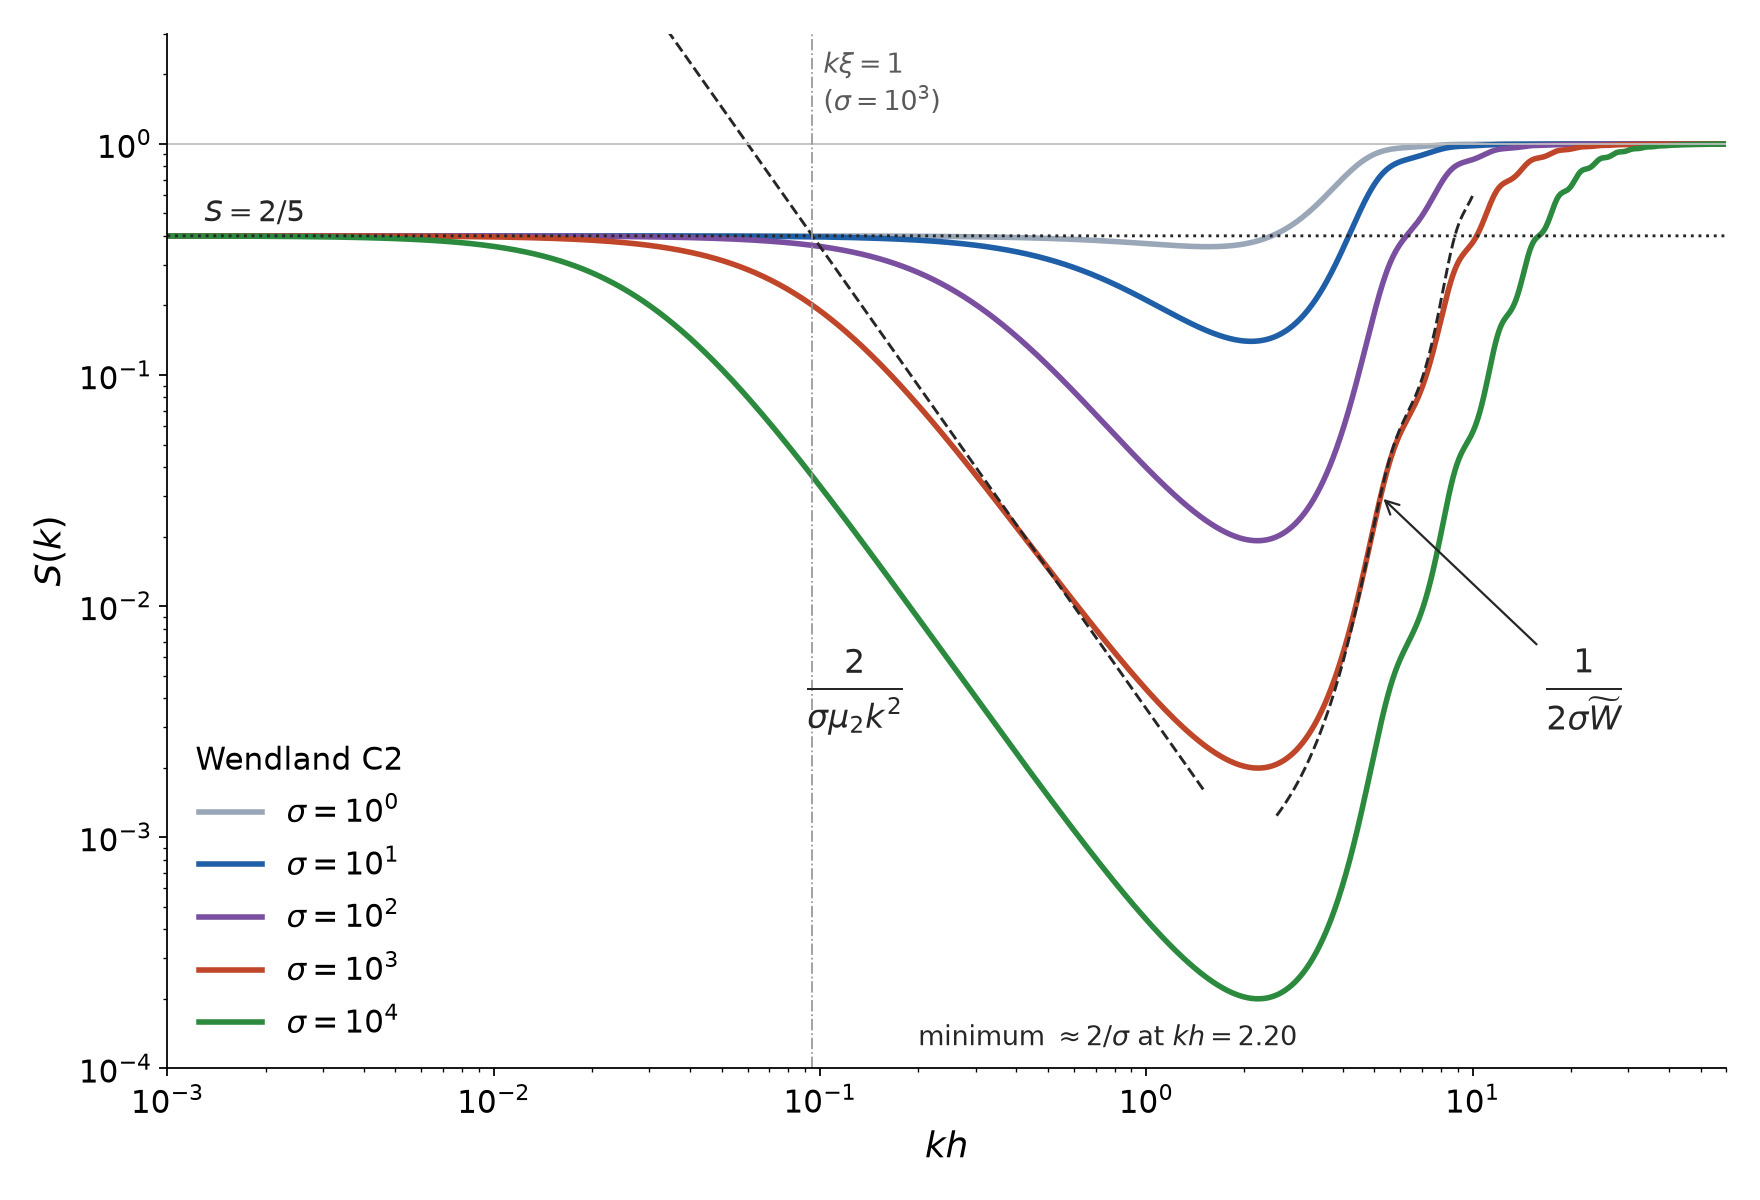
\includegraphics[width=0.7\textwidth]{figs/sk_regimes.png}
\caption{\Eq{Sk} for Wendland C2 at $\sigma=1$--$10^4$; dashed, the asymptotes at $\sigma=10^3$.  (C4 and C6: \texttt{figs/sk\_regimes\_C4.png},
\texttt{\_C6.png}.)  Script: \texttt{examples/sk\_regimes.py}.}
\label{fig:skreg}
\end{figure}

\subsection{The scales in $g(r)$}

\st
\bar nh^2\,[g(r)-1]=F(r/h;\sigma)=\frac{h^2}{2\pi}\int_0^\infty k\,dk\,J_0(kr)\,[S(k)-1],
\stp
with $J_0$ the Bessel function, has three scales (\Fig{fig:grreg}).
\begin{itemize}
\item \emph{The core}, $r\lesssim1/k_*$: $F(0)\approx-(k_*h)^2/4\pi$, from $-1.4$ at $\sigma=4$ to $-36$ at $\sigma=13500$ (C2).
\item \emph{The kernel}, $r\approx h$ to $4h$: the hole closes by $r\approx0.6h$; the structure at $2h$--$4h$ is the edge of the support of $W$ and $W*W$.
\item \emph{The label-correlation length}: for $r\gg h$ the Ornstein--Zernike form gives a positive halo,
\st
\bar n\,[g(r)-1]\simeq\frac{1/(1+\alpha)}{2\pi\xi^2}\,K_0(r/\xi)=\frac{K_0(r/\xi)}{\pi\sigma\mu_2},\qquad
\sigma\,\bar nh^2[g-1]\simeq\frac9{5\pi}K_0(r/\xi)\ \ (\text{C2}),
\stp
of order $10^{-3}$ in $g-1$ at the parameters of the runs.
\end{itemize}
The halo shows in the running integral, the excess number of particles within $R$ of a particle,
\st
N(R)=\bar n\int_{r<R}d^2r\,[g(r)-1]=R\int_0^\infty dk\,J_1(kR)\,[S(k)-1],
\stp
which depends on $\sigma$ only (\Fig{fig:running}): it falls to $-1$ across the hole and returns to $-1+S(0)=-\alpha/(1+\alpha)$ across $\xi$.  The
HMC points for $h/a=2$, $3$, $4$ fall on one curve, as predicted; the return at $\sigma=179$ needs $g(r)$ to $R\approx10h$, and the runs record it
only to $2h$.

\begin{figure}[h]
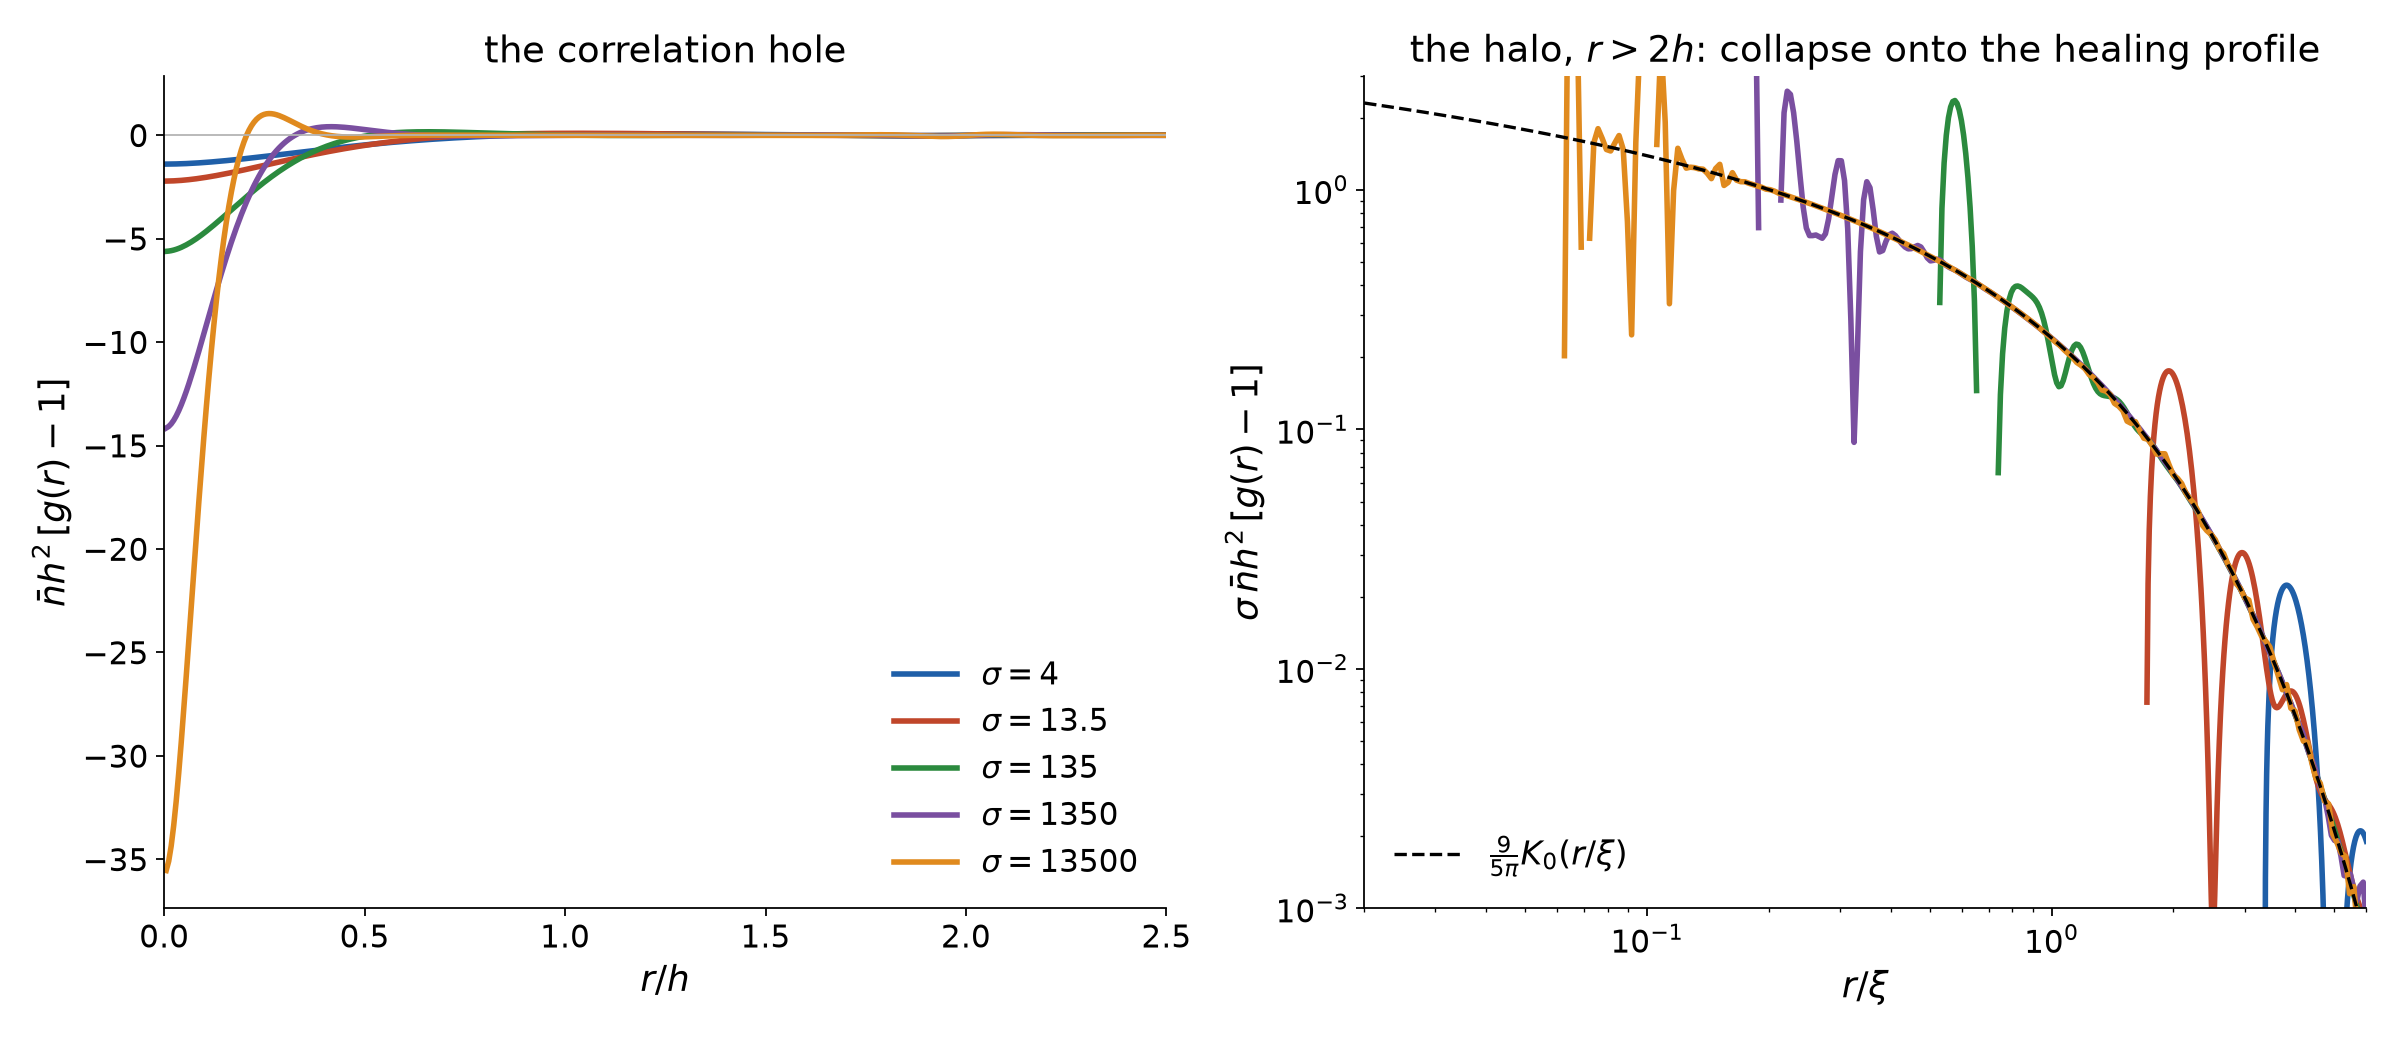
\includegraphics[width=0.85\textwidth]{figs/gr_regimes.png}
\caption{Gaussian theory, C2.  Left: the hole, $\bar nh^2(g-1)$.  Right: $\sigma\bar nh^2(g-1)$ for $r>2h$ against $r/\xi$, on the Ornstein--Zernike profile
$(9/5\pi)K_0$.  Script: \texttt{examples/gr\_regimes.py}.}
\label{fig:grreg}
\end{figure}

\begin{figure}[h]
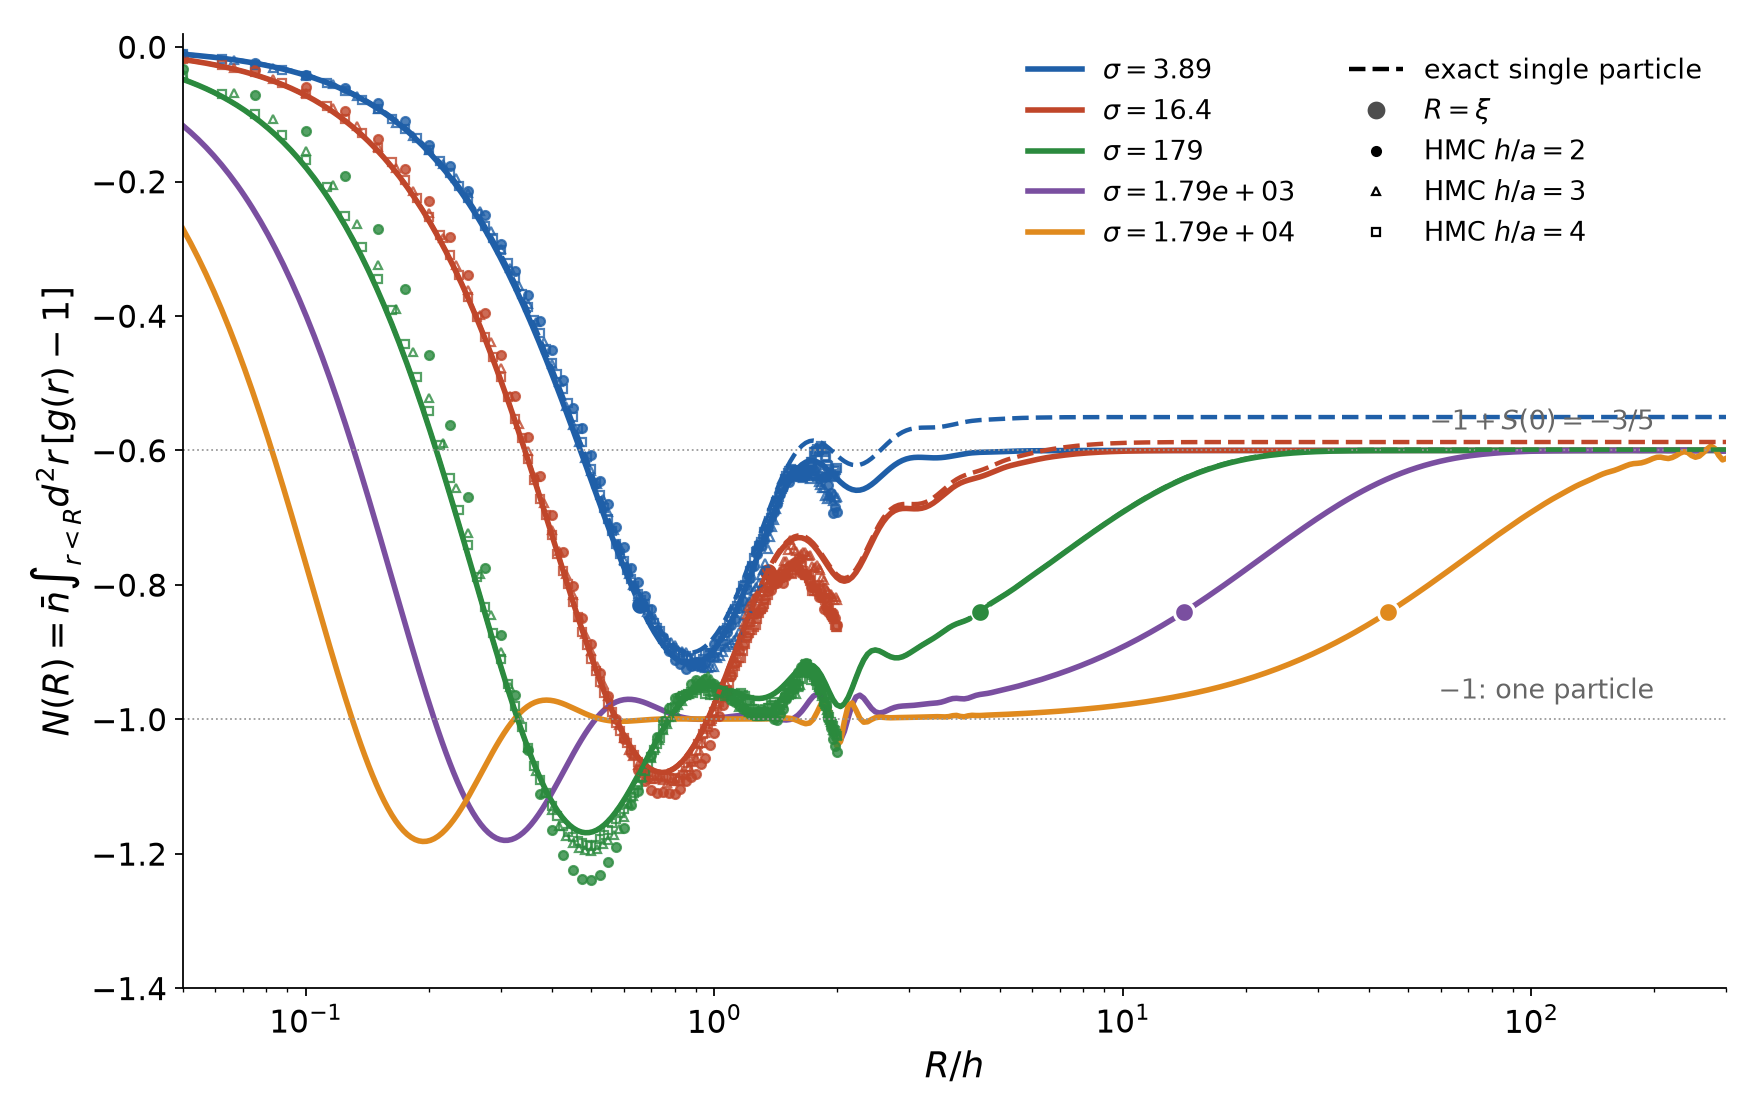
\includegraphics[width=0.7\textwidth]{figs/running_integral.png}
\caption{The running integral $N(R)$: Gaussian theory (solid; dots at $R=\xi$) at $\sigma(T_0)$ of the three runs and at two larger $\sigma$, HMC (symbols, to
$R=2h$), and for the three runs the improved theory with the exact single particle (dashed), whose plateau is $-1+S(0)=-\alpha_{\rm eff}/(1+\alpha_{\rm eff})=-0.55$
at $\sigma=3.9$.  Script: \texttt{examples/running\_integral.py}.}
\label{fig:running}
\end{figure}

\subsection{The logarithm is special to $d=2$}

The logarithm of \Eq{Vlog} comes from the middle regime, where $\widetilde W\simeq1$ and $S\simeq2/(\sigma\mu_2k^2)$:
\st
\frac{\avg{\delta V_a^2}}{V^2}\supset\frac1{\bar n}\int_{1/\xi}^{1/h}\frac{d^dk}{(2\pi)^d}\,\frac{2}{\sigma\mu_2k^2}\;\propto\;\frac1{\sigma\bar n}\int_{1/\xi}^{1/h}k^{d-3}\,dk .
\stp
The $1/k^2$ is generic ($1-\widetilde W\propto k^2$); the counting depends on $d$.
\begin{center}
\begin{tabular}{cccc}
\toprule
$d$ & integrand & dominated by & variance $\times\,\sigma\bar nh^d$ \\
\midrule
1 & $dk/k^2$ & $k\sim1/\xi$ & $\xi/h\propto\sqrt\sigma$ \\
2 & $dk/k$ & every decade between $h$ and $\xi$ & $\ln(\xi/h)\propto\ln\sigma$ \\
3 & $dk$ & $k\sim1/h$ & constant \\
\bottomrule
\end{tabular}
\end{center}
$d=2$ is marginal, as for the two-dimensional Coulomb logarithm.  Because the logarithm reaches out to $\xi$, a box smaller than $\xi$ cuts it
off: by up to $33\%$ at $\sigma=179$ in $L=9h$.

\subsection{Does the fluid know about $\xi$?}

Almost not.  At fixed positions each particle's entropy fluctuates by \Eq{intrinsic} about its mean $sV_a$.  For the point sum
$S_{\bm k}=\sum_as_ae^{-i\bm k\cdot\bm x_a}$ the fluctuations of the particles add to $C_V\sum_aV_a=C_VL^2$, whatever the positions, and the mean
part, $s\int\rho/n\,e^{-i\bm k\cdot\bm x}$, gives to linear order $s(1-\widetilde W)\delta\rho_{\bm k}/\bar n$ (for the smoothed density,
$s\widetilde W(1-\widetilde W)\delta\rho_{\bm k}/\bar n$).  So, with $s^2/(\bar nC_V)=c_s^2s_a$ for a constant $c_s^2=s/C_V$,
\st
\frac{\avg{|S_{\bm k}|^2}}{L^2C_V}=1+c_s^2\,s_a\,(1-\widetilde W)^2S(k),
\label{leak}
\stp
and the leak of the positions relative to the fluid's own fluctuations is, at $kh\ll1$ ($c_s^2s_a=(1+c_s^2)\sigma$),
\st
(1+c_s^2)\,\frac{\mu_2k^2}8\,\frac{\xi^2k^2}{1+\xi^2k^2}\le(1+c_s^2)\,\frac{\mu_2k^2}8 .
\stp
The momentum at rest does not see the positions at all: $\avg{\bm m_a}=0$, and $\avg{|\bm M_{\bm k}|^2}$ per component is $\widetilde W^2(e+p)TL^2$.
The equal-time hydrodynamic correlators at $kh\ll1$ are those of the continuum, filtered by $\widetilde W^2$.  HMC follows \Eq{leak} within errors
at $\sigma=16.4$ and $179$; at $\sigma=3.9$ it needs the exact single particle (\Fig{fig:leak}).

\begin{figure}[h]
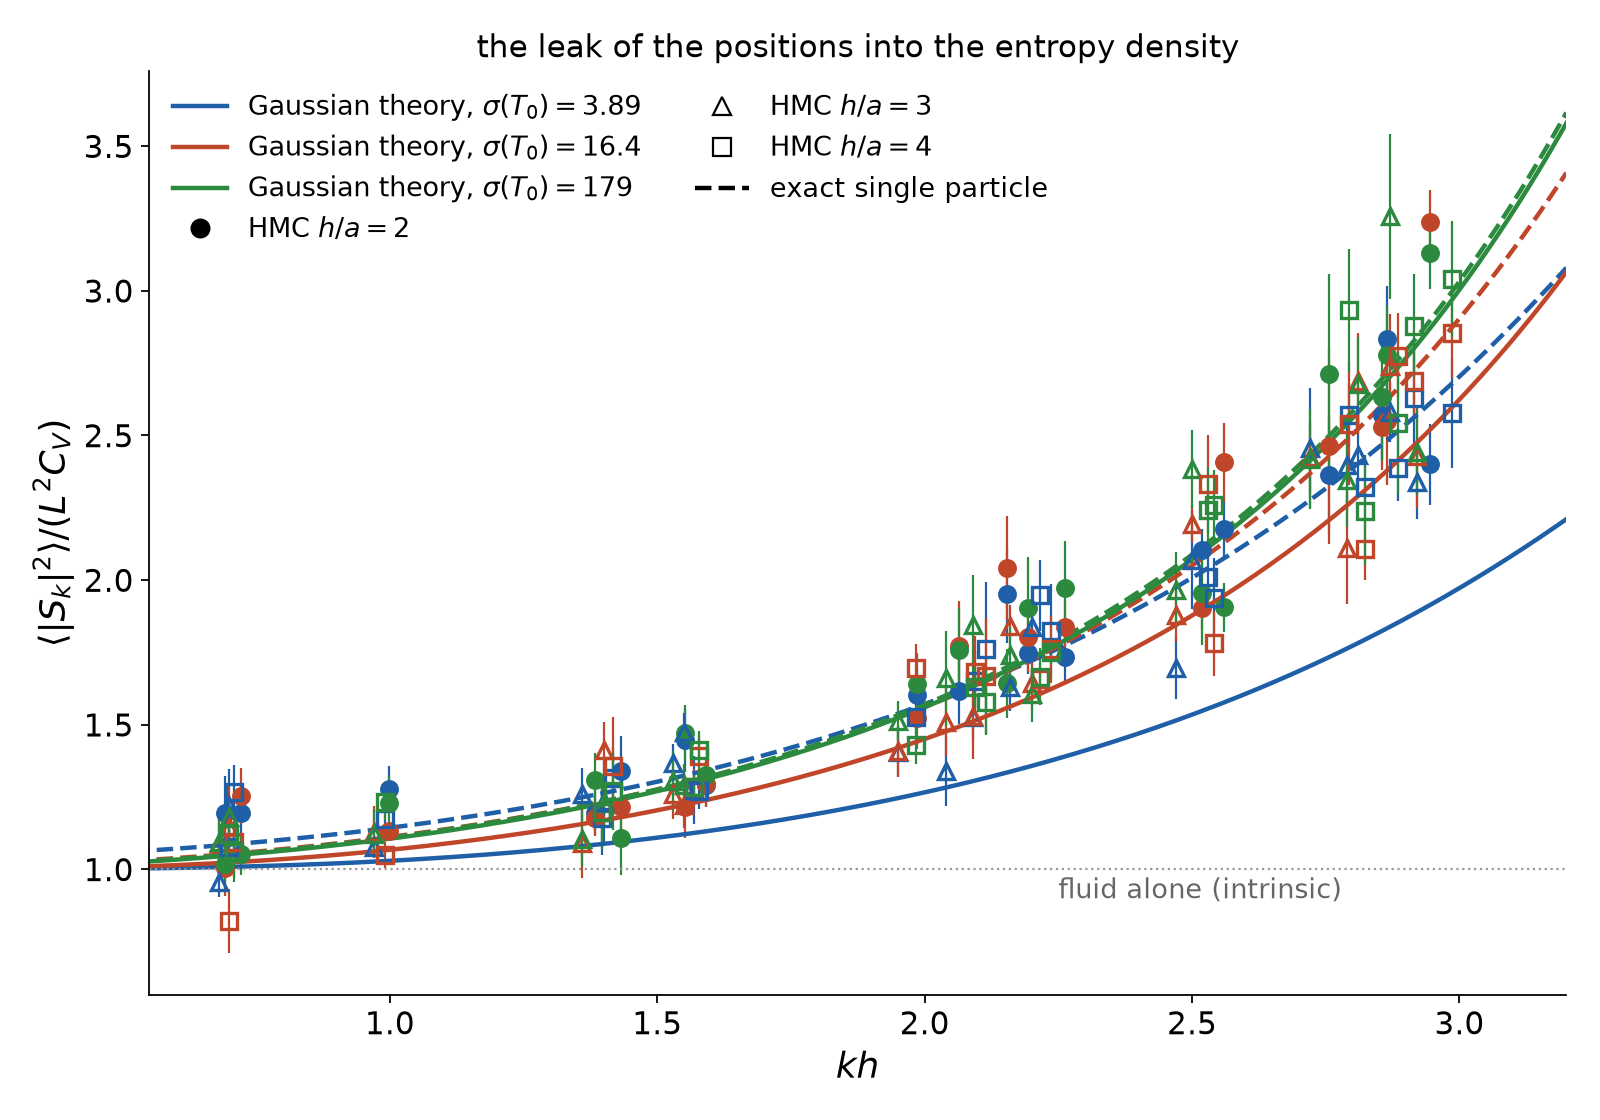
\includegraphics[width=0.7\textwidth]{figs/entropy_leak.png}
\caption{$\avg{|S_{\bm k}|^2}/(L^2C_V)$, with $C_V$ at $T_0$, the nine HMC runs (errors from eight blocks) against \Eq{leak} with $c_s^2=1/2$ at $\sigma(T_0)$ (solid)
and the improved theory (dashed): the exact single particle, the intrinsic part $r_s\avg{V_a}\bar n$ plus the leak through $\avg{s|V'}=s_{\rm off}+bV'/V$
(\App{app:misses}).  The dotted line at $1$ is the fluid alone.  Script: \texttt{examples/entropy\_leak.py}.}
\label{fig:leak}
\end{figure}

\paragraph{The momentum.}  At rest each particle's mean momentum is zero, and at fixed positions the particles are independent with
\Eq{intrinsic}, so for the point sums $\bm M_{\bm k}=\sum_a\bm m_ae^{-i\bm k\cdot\bm x_a}$, projected along $\bm k$ (longitudinal) or across it (transverse),
\st
\frac{\avg{|M_{\bm k}|^2}}{L^2\,T(e+p)}=\frac{\sum_aV_a}{L^2}=\avg{V_a}\bar n ,
\label{Mpred}
\stp
flat in $k$, the same for both projections and every $\sigma$, and below $1$ by at most $3\%$ (Table~\ref{tab:hmc}): the positions do not leak into the
momentum at all.  HMC (\Fig{fig:mom}) is flat in $k$ and the same for both projections, as predicted, but its level depends on $\sigma$: averaged over
$k$, $1.49$--$1.58$ at $\sigma=3.9$, $1.11$--$1.14$ at $\sigma=16.4$, and $0.99$--$1.03$ at $\sigma=179$, the same at every $h/a$.  The miss is in the single-particle
variance, not in the positions: the improved theory (dashed in \Fig{fig:mom}, \App{app:misses}) accounts for it.

\begin{figure}[h]
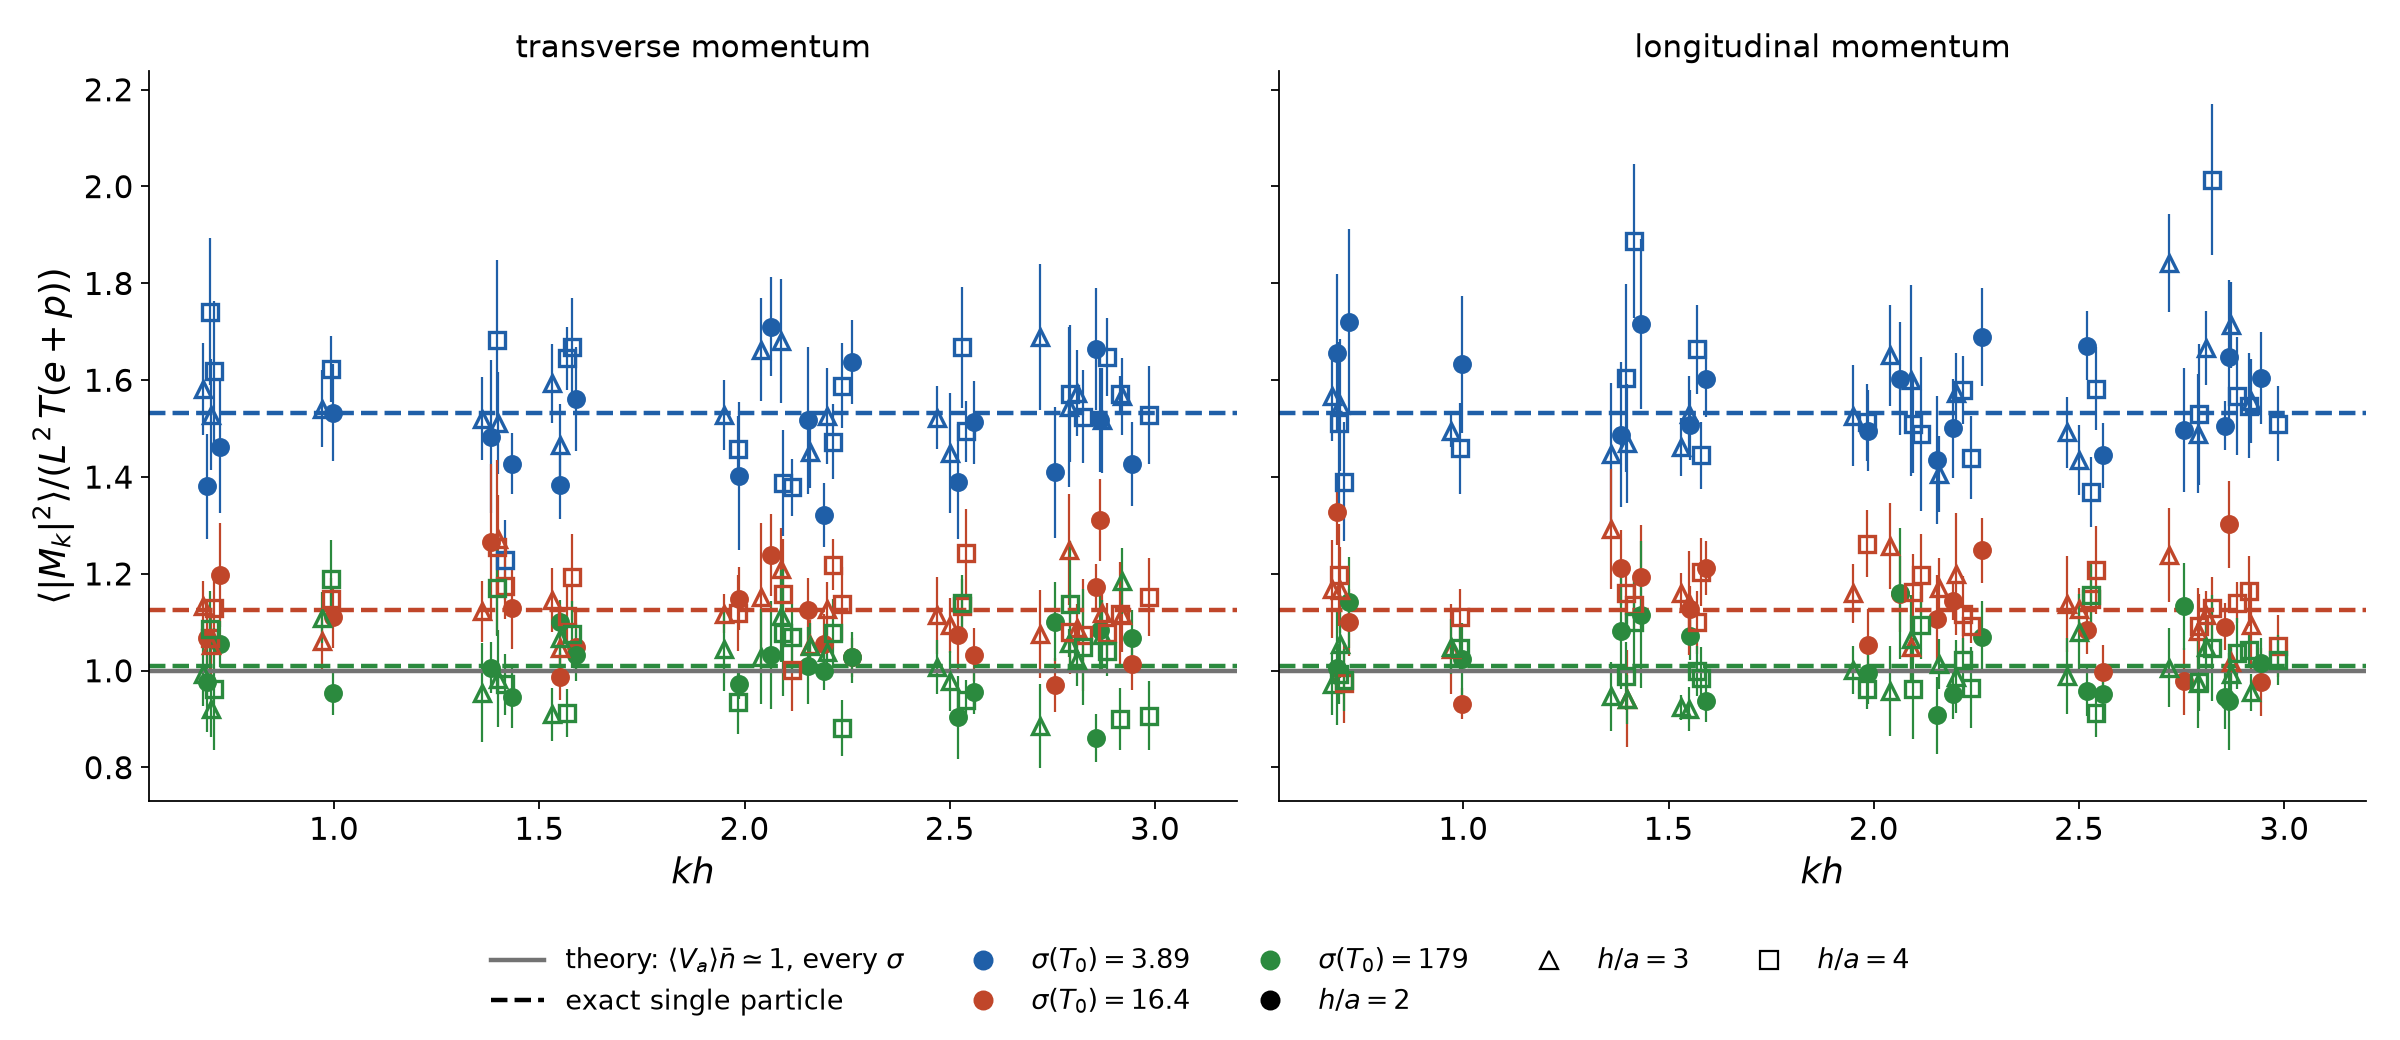
\includegraphics[width=\textwidth]{figs/momentum_fluct.png}
\caption{$\avg{|M_{\bm k}|^2}/(L^2T(e+p))$, with $T=T_0$ and $e+p=T_0s(T_0)$, transverse (left) and longitudinal (right), the nine HMC runs (errors from eight blocks)
against \Eq{Mpred} (solid) and the improved theory (dashed): the exact single particle at $T_0$, $r_m\avg{V_a}\bar n$.
Script: \texttt{examples/momentum\_fluct.py}.}
\label{fig:mom}
\end{figure}

\subsection{What $\alpha$ counts: the renormalized equation of state}
\label{app:alpha}

The point: $\alpha$ is not visible in a continuum fluid, but it is physical; it belongs to the difference between the equation of state put into the
model (the bare one) and the thermodynamics the model actually has (the renormalized one).

\paragraph{What $\alpha$ counts.}  A particle carries the conserved densities of the fluid, its entropy (or energy) and $d$ components of momentum.  Each is
extensive and fluctuates thermally with a width $\propto\sqrt{V_a}$, \Eq{intrinsic}, so the number of distinguishable fluctuation states of a particle grows as
$V_a^{(d+1)/2}$:
\st
\alpha=\tfrac12\times(\text{number of conserved densities per particle}),
\stp
$(d+2)/2$ with a conserved charge.  $\alpha\ln V_a$ is the Einstein fluctuation entropy of a subsystem of volume $V_a$, $\tfrac12\ln\det(\chi V_a)$.  $\sigma$ is the maximum of
$\Phi_a$, of order $s_a$; $\alpha$ is its Gaussian width, of order one: the $1/s_a$ correction to the thermodynamics of a particle.

\paragraph{Why a continuum fluid does not see it.}  Its direct signature, $S(0)=1/(1+\alpha)$, is a property of the labels, which the fluid fields barely see.
Its thermodynamic partners, the entropy $\alpha\ln V_a$ and the energy $\Delta e$ of \Eq{Deltae} per particle, are per unit volume of order
\st
\bar n\,\Delta e\sim T\,\bar n\sim T\Lambda^d ,
\stp
with the density of particles as the cutoff, $\Lambda^d\sim\bar n$.  These are the cutoff-dependent terms of fluctuating hydrodynamics, the one-loop $\tfrac12\mathrm{Tr}\ln\chi$ of
the fluctuations of the conserved densities, which are absorbed into the renormalized equation of state; only the renormalized one is measured.

\paragraph{In the model.}  The cutoff is explicit and the input equation of state is the bare one, so the absorbed terms appear as differences of order $1/s_a$
between the input and the model's own thermodynamics, which follows from $\ln Z_a$.  For example the energy density of the model at the temperature $T$ is
\st
e_{\rm ren}(T)=\bar n\avg{e_a}_T=e(T)+\bar n\,\Delta e(T),
\stp
which is why the bath temperature of the runs is below $T(S_0)$ (\Sect{sec:test}), and the momentum susceptibility is $r_mT(e+p)$, $r_m=1.57$ at $s(T)V=11.7$ (\App{app:misses};
there from the full single-particle distribution, not from $\alpha$ alone, but of the same order).  A comparison with continuum hydrodynamics is consistent
either at $s_a\gg1$, where these terms vanish, or against the model's renormalized thermodynamics, as in \App{app:misses}.  In the continuum limit at fixed
$s\,h^2$ (\App{app:continuum}) $s_a$ falls and the cutoff terms grow, as $T\Lambda^d$ does; holding the renormalized equation of state fixed would need a
counterterm in the bare one.

\subsection{The continuum limit}
\label{app:continuum}

The physical limit holds the fluid fixed ($s$, $T$, and so $p/T$) and the kernel $h$ in physical units, and adds particles.  Then $\sigma$ is not
fixed.  The fixed combinations are the content of a kernel area,
\st
\sigma\,\bar nh^2=\frac pT\,h^2,\qquad s_a\,\bar nh^2=s\,h^2,
\stp
so that
\st
\sigma=\frac{(p/T)\,h^2}{\bar nh^2},\qquad s_a=\frac{s\,h^2}{\bar nh^2}
\stp
both fall as $1/\bar nh^2$.  The number of particles is a numerical parameter; the physical one is $s\,h^2$, which sets the size of the fluid's own
fluctuations in a kernel.

\paragraph{What adding particles does at fixed $s\,h^2$.}
\begin{itemize}
\item The equal-time fluid correlators do not change: the fluid's own part depends on $s\,h^2$ only, and the leak of the positions,
  $(1+c_s^2)\mu_2k^2/8$, does not depend on $\sigma$.
\item The pair correlation flattens, $g-1\propto1/(\bar nh^2)$.
\item The volume variance, \Eq{Vlog}, falls only through its logarithm,
  \st
  \frac{\avg{\delta V_a^2}}{V^2}\sim\frac1\pi\,\frac{\ln\sigma}{(p/T)\,h^2} .
  \stp
\item The label-correlation length shrinks, $\xi^2/h^2=\sigma\mu_2/(2(1+\alpha)h^2)$; once $\xi<h$ the middle regime of $S(k)$ is gone and the positions are a label gas
  with $S(0)=1/(1+\alpha)$ on every scale above $h$.
\item $S(0)=1/(1+\alpha)$ does not change (at large $s_a$; at small $s_a$, $\alpha\to\alpha_{\rm eff}$, \App{app:misses}).
\end{itemize}

\paragraph{A window, not a limit.}  The theory, and the particle description, need both approximations of \App{app:expand}:
\st
1\;\ll\;\bar nh^2\;\ll\;s\,h^2\qquad\Longleftrightarrow\qquad \bar nh^2\gg1\ \text{and}\ s_a\gg1 .
\stp
Adding particles at fixed $s\,h^2$ lowers $s_a$ and raises the corrections \Eq{Zcorr}; at $s_a\sim1$ a particle is no longer a thermodynamic fluid element.
So the limit is $s\,h^2\to\infty$ (the kernel holds many quanta: the hydrodynamic condition), with $\bar nh^2$ in the window.

\paragraph{The runs.}  The nine runs vary $h/a$ at fixed $s_a$, i.e.\ at fixed $\sigma$, so a larger $h/a$ also has a larger $s\,h^2$: they are not
the physical limit.  A comparison at fixed $s\,h^2$ runs along a diagonal, e.g.
\st
s_a\,\bar nh^2:\qquad (h/a=2,\ s_a=541)\to2500,\qquad (h/a=4,\ s_a=135)\to2500,
\stp
the second not run.  The nearest pair in hand is $(h/a=4,\ s_a=16)$ at $296$ and $(h/a=2,\ s_a=54)$ at $249$.

\subsection{The bath temperature and the exact single particle}
\label{app:misses}

The point: at small $\sigma$ the saddle point of a particle's weight is not enough, and the constants of the theory must be those of the ensemble's
temperature.  With both, the theory has no free parameter left (\texttt{statics.tex}, Step 0).  In the first version of this note (at $c_s^2=1/3$) the runs were compared
with \Eq{Sk} at the $\sigma$ of the start, and at the smallest $\sigma$ four quantities missed by $14$--$23\%$; this appendix is the account of those misses.

\paragraph{The bath temperature.}  The runs start on the lattice with the entropy density $S_0=s_a/V$ at rest, and hybrid Monte Carlo samples
the canonical ensemble at the temperature $T_0$ whose mean energy is that of the start.  The fluctuations of each particle hold the energy $\Delta e=5\,T_0$
of \Eq{Deltae}, so $T_0$ is below $T(S_0)$:
\st
\frac{T_0}{T(S_0)}=0.855,\ 0.955,\ 0.996\qquad(s_a=16,\ 54,\ 541\ \text{at the start}).
\stp
Every constant of the ensemble belongs to $T_0$: $\sigma=p(T_0)/(T_0\bar n)=3.89$, $16.4$, $179$ (not $s_a/3=5.3$, $18$, $180$); $w=T_0s(T_0)$; $C_V(T_0)$.

\paragraph{The exact single particle.}  At $T_0$ and $V=1/\bar n$ the quadrature of the single-particle distribution (\texttt{examples/single\_particle.jl},
Liouville measure) gives, beyond the saddle point,
\begin{center}
\begin{tabular}{cccccccc}
\toprule
$\sigma(T_0)$ & start $s_a$ & $s(T_0)V$ & $\sigma_{\rm eff}$ & $\alpha_{\rm eff}$ & $r_s$ & $r_m$ & $\avg{s_a}/s(T_0)V$ \\
\midrule
3.89 & 16 & 11.7 & 4.02 & 1.225 & 0.918 & 1.568 & 1.26 \\
16.4 & 54 & 49.2 & 16.44 & 1.425 & 0.969 & 1.140 & 1.07 \\
179 & 541 & 536 & 178.8 & 1.493 & 0.997 & 1.013 & 1.01 \\
\bottomrule
\end{tabular}
\end{center}
with $\alpha_{\rm eff}$ and $\sigma_{\rm eff}$ from the fit of the exact $\ln Z_a$ by the form of its saddle point, $\ln Z_a(V')\simeq\alpha_{\rm eff}\ln V'+\sigma_{\rm eff}V'/V$
near $V=1/\bar n$,
\st
\alpha_{\rm eff}=-V^2\frac{d^2\ln Z_a}{dV^2},\qquad\sigma_{\rm eff}=V\frac{d\ln Z_a}{dV}+V^2\frac{d^2\ln Z_a}{dV^2},
\stp
the effective phase-space exponent and volume coefficient of a particle, which tend to $\alpha=(d+1)/2=3/2$ and $\sigma=p/(T\bar n)$ at large $s_a$, and $r_s$, $r_m$
the entropy and momentum variances at fixed volume over $C_VV$ and $T(e+p)V$.  The momentum variance is $57\%$ above the Gaussian at $s(T_0)V=11.7$: the
relativistic tail.  The light cone cuts the momentum off, and the particle has fewer effective phase-space dimensions: $\alpha_{\rm eff}=1.225$ at $\sigma=3.9$.
\Eq{Sk} keeps its form with $\alpha,\sigma\to\alpha_{\rm eff},\sigma_{\rm eff}$,
\st
S(k)=\frac1{1+2\alpha_{\rm eff}\,\widetilde W(1-\tfrac12\widetilde W)+2\sigma_{\rm eff}\,\widetilde W(1-\widetilde W)},\qquad S(0)=\frac1{1+\alpha_{\rm eff}}=0.449,\ 0.412,\ 0.401 ,
\stp
and the labels are an ideal gas with $\mu_{\rm label}=(1+\alpha_{\rm eff})T\ln n$.

\paragraph{Against hybrid Monte Carlo} (\texttt{examples/single\_particle\_compare.py}, \Fig{fig:step0}), with no free parameter:
\begin{itemize}
\item the momentum correlator, $r_m\avg{V_a}\bar n$: HMC/prediction $0.99$--$1.01$ at every $\sigma$ and $h/a$;
\item the entropy correlator, the intrinsic part $r_s$ plus the leak through the exact $\avg{s|V}$ (which has an offset, $\avg{s|V'}=s_{\rm off}+bV'/V$,
  $s_{\rm off}\approx2.7$ at $\sigma=3.9$): $0.99$--$1.01$;
\item $S(k)$ on the box modes: $0.98$--$1.03$ (against \Eq{Sk} with $\alpha=3/2$ at $\sigma(T_0)$, $1.03$--$1.08$ at $\sigma=3.9$; at the $\sigma$ of the start, $1.19$--$1.24$);
\item the volume variance ($10^3\bar n^2\avg{\delta V_a^2}$, data against the exact theory in the box): $16.4/17.2$, $7.32/7.64$, $4.35/4.30$ at $\sigma=3.9$ and $h/a=2,3,4$;
  $7.33/7.99$, $3.68/3.55$, $1.93/2.00$ at $16.4$; $1.03/1.12$, $0.50/0.50$, $0.29/0.28$ at $179$.  The theory is $8\%$ high at $h/a=2$ ($\bar nh^2=4.6$) and
  within $\pm4\%$ at $h/a=3$ and $4$.
\end{itemize}
So the misses were the bath temperature and the single-particle distribution; approximation 1 of \App{app:expand} is replaced by the exact
quadrature, and what is left is approximation 2 (few neighbours) and 3 (the volume variance).  The Einstein measure gives the same $r_m$, $\alpha_{\rm eff}$,
$\sigma_{\rm eff}$ within $1\%$, and $r_s$ lower by $4\%$ at $\sigma=3.9$.

\begin{figure}[h]
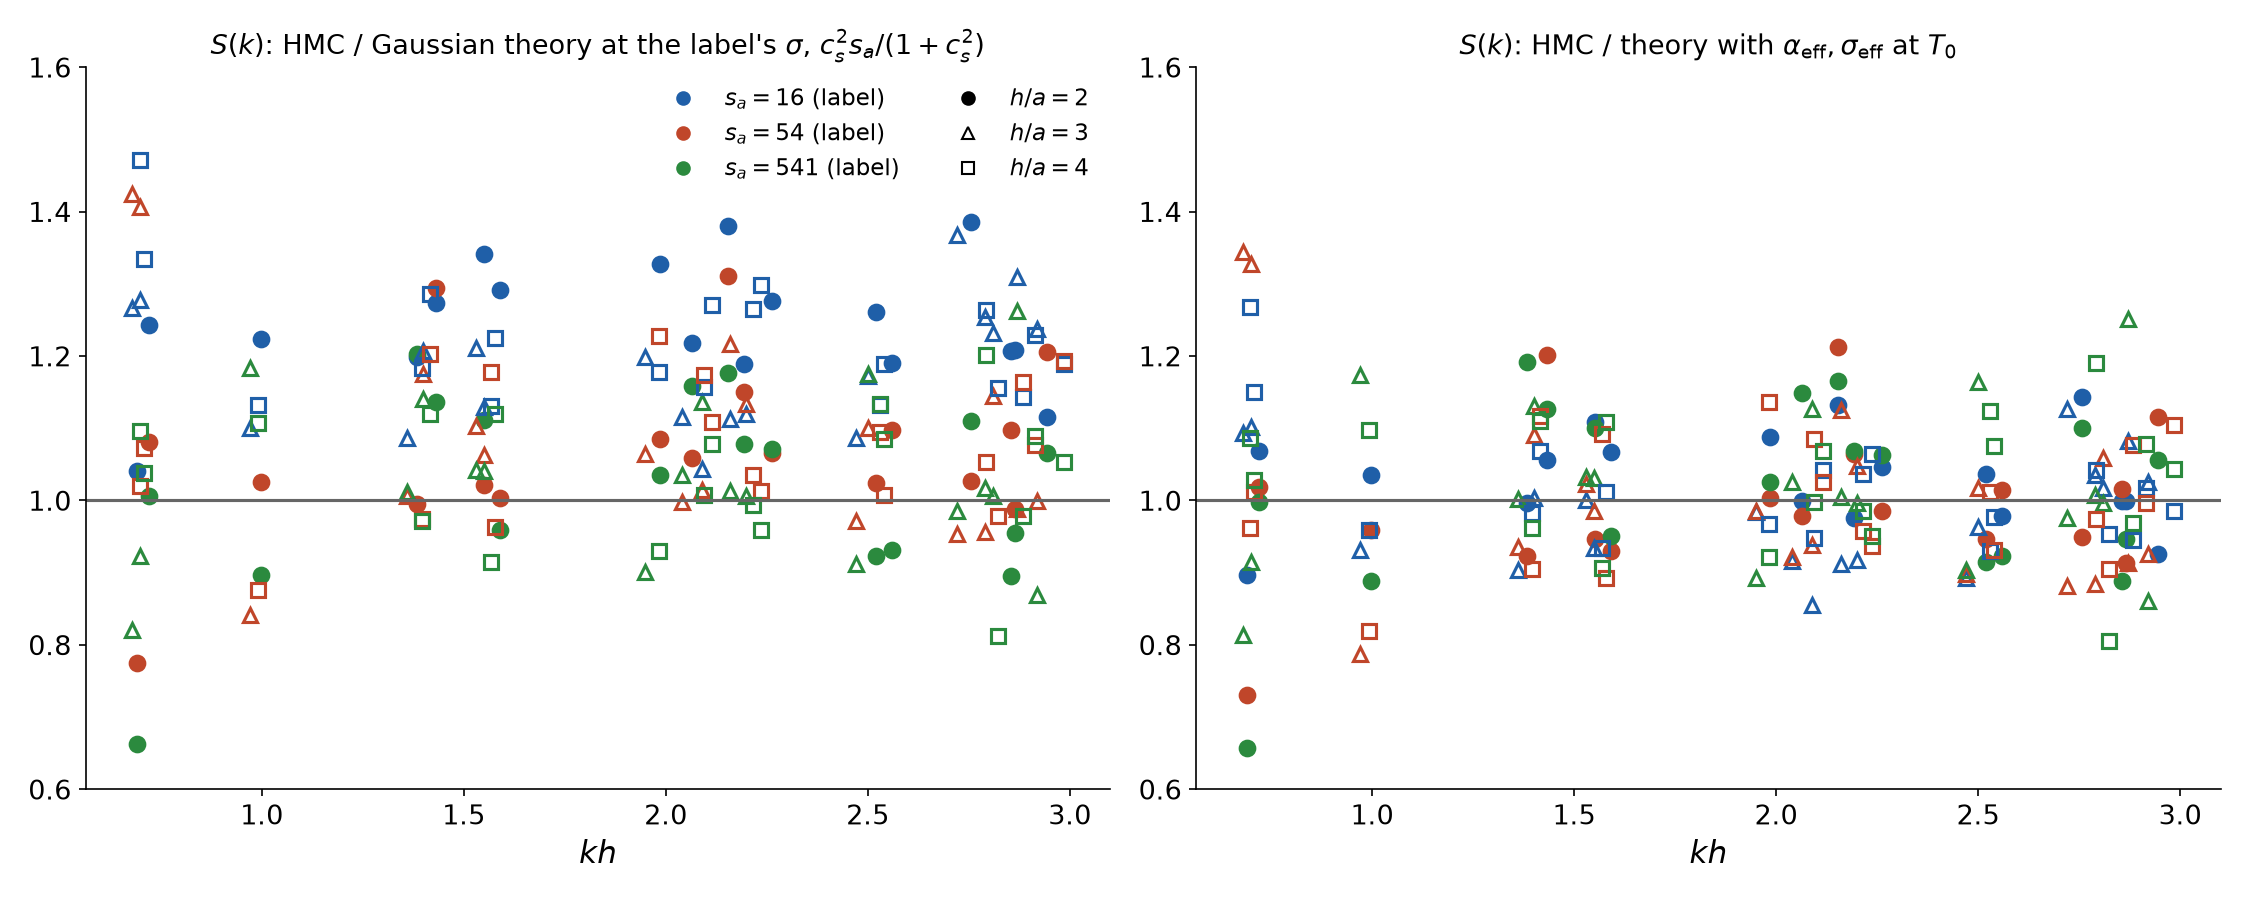
\includegraphics[width=\textwidth]{figs/step0_positions.png}
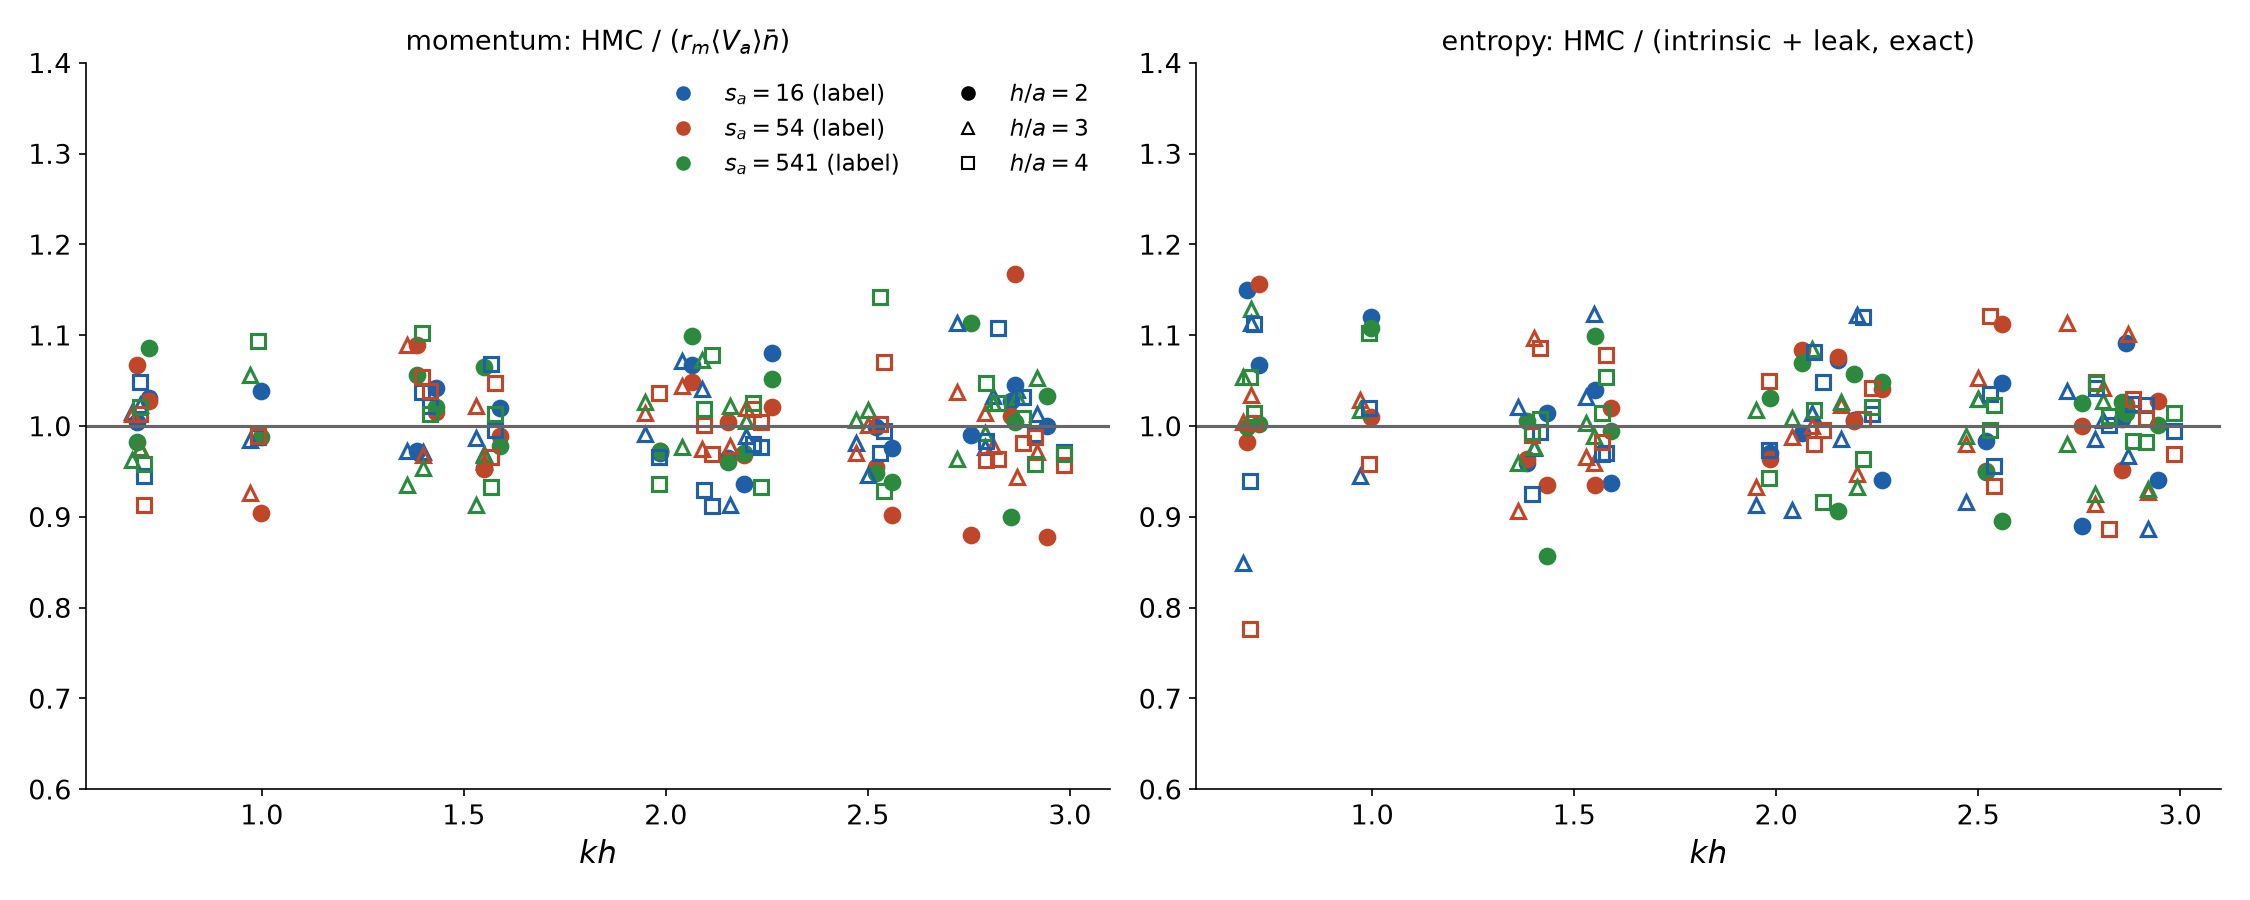
\includegraphics[width=\textwidth]{figs/step0_momentum_entropy.png}
\caption{The nine HMC runs over the predictions.  Top: $S(k)$ against the Gaussian theory at the $\sigma$ of the start, $c_s^2s_a/(1+c_s^2)=s_a/3$ (left), and with
$\alpha_{\rm eff},\sigma_{\rm eff}$ at $T_0$ (right).  Bottom: the momentum and entropy correlators against the exact single particle at $T_0$.  Colours by the
start's $s_a=16$, $54$, $541$, i.e.\ $\sigma(T_0)=3.9$, $16.4$, $179$.  Script: \texttt{examples/single\_particle\_compare.py}.}
\label{fig:step0}
\end{figure}

\subsection{The kernels}

\begin{figure}[h]
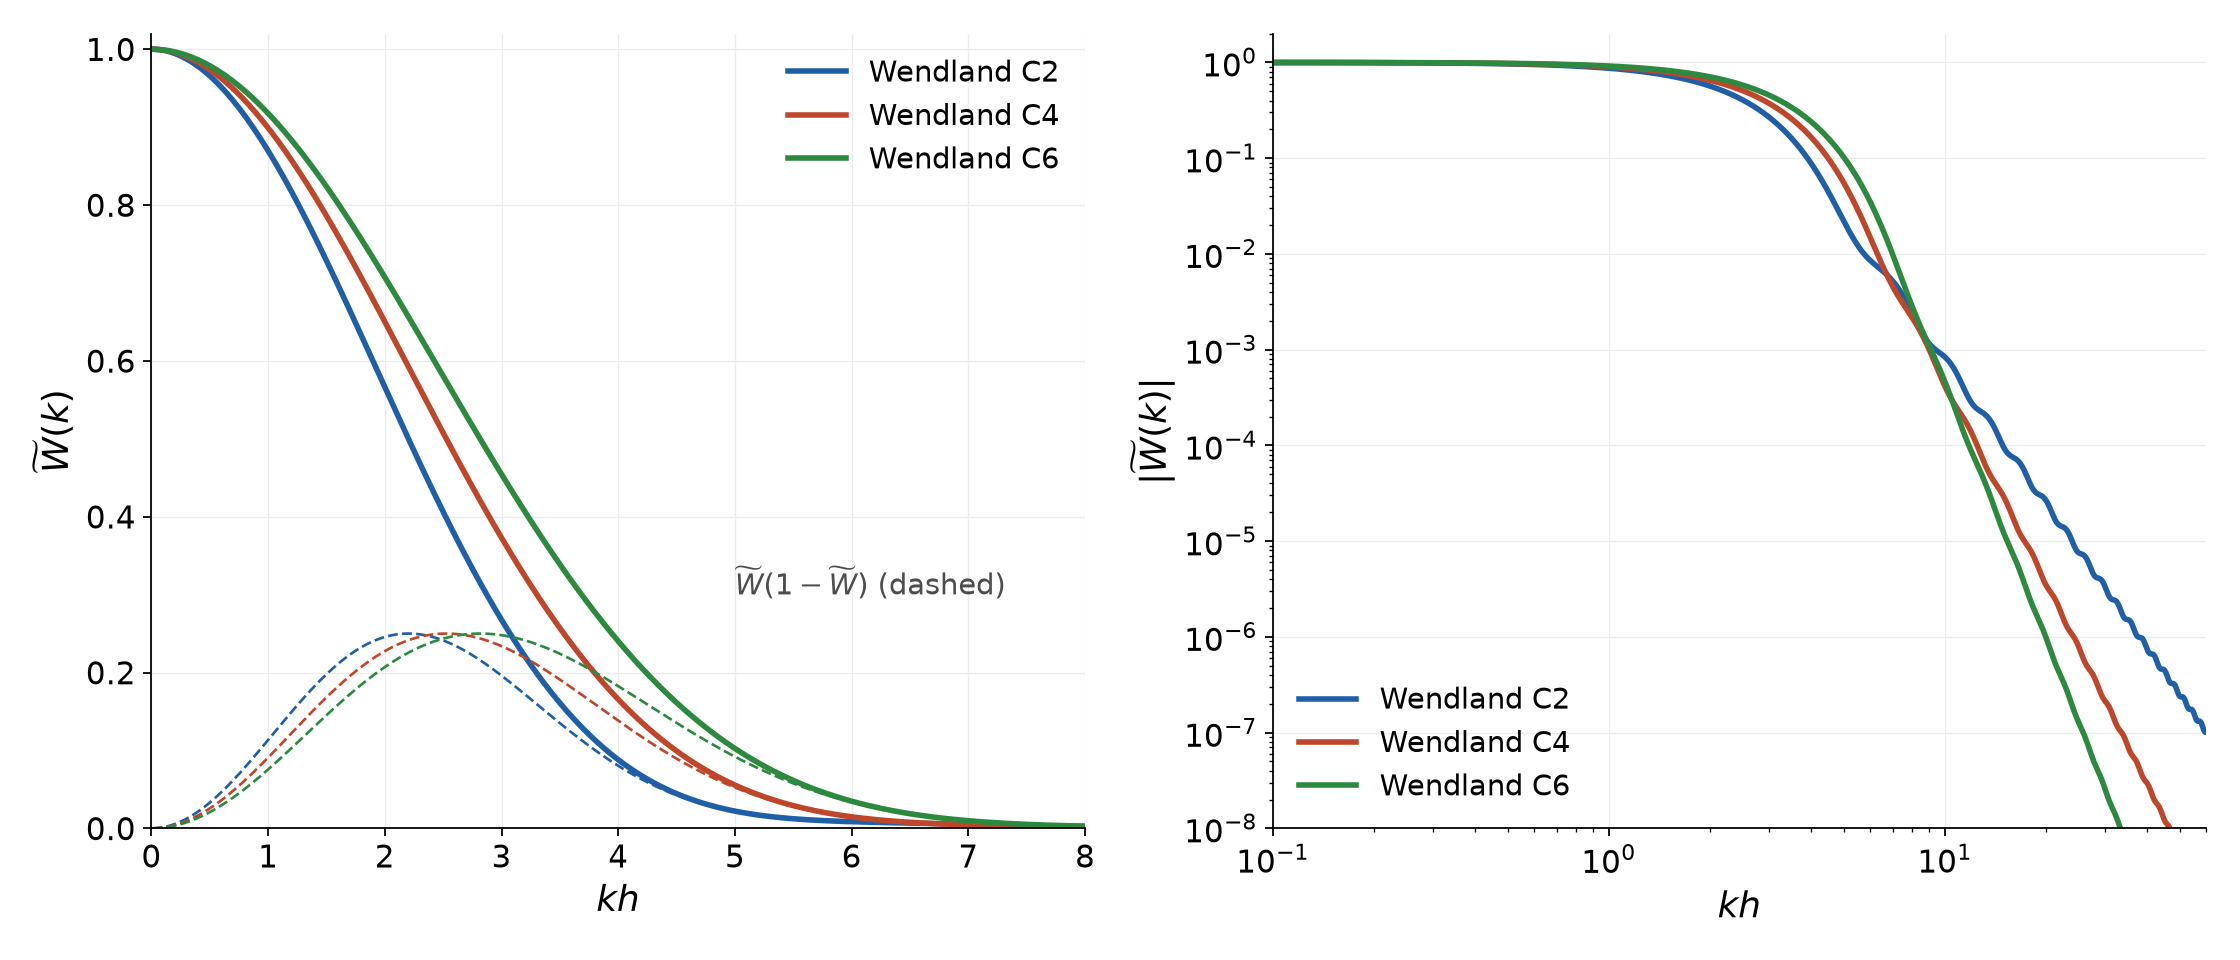
\includegraphics[width=0.85\textwidth]{figs/wendland_ft.png}
\caption{The Fourier transforms of the two-dimensional Wendland kernels (support $2h$, $\widetilde W(0)=1$), with $\widetilde W(1-\widetilde W)$ dashed.
All are positive, so every mode of \Eq{Ak} is stable.  Script: \texttt{examples/wendland\_ft.py}.}
\label{fig:wft}
\end{figure}

\end{document}
